\chapter{Guiding Soft Robots with Motor-Imagery Brain Signals}
\label{chp:braincontrol}

\begin{abstract}
    Integrating Brain-Machine Interfaces into non-clinical applications like robot motion control remains difficult - despite remarkable advancements in clinical settings. Specifically, EEG-based motor imagery systems are still error-prone, posing safety risks when rigid robots operate near humans. This chapter presents an alternative pathway towards safe and effective operation by combining wearable EEG with physically embodied safety in soft robots. We introduce and test a pipeline that allows a user to move a soft robot's end effector in real time via brain waves that are measured by as few as three EEG channels. A robust motor imagery algorithm interprets the user's intentions to move the position of a virtual attractor to which the end effector is attracted, thanks to a Cartesian impedance controller. We specifically focus here on planar soft robot-based architected metamaterials. Due to their compact and portable nature, they could be in the future mounted to a mobile platform and allow assistance with activities of daily living. We preliminarily but quantitatively evaluate the approach on the task of setpoint regulation. We observe that the user reaches the proximity of the setpoint in 66\% of steps and that for successful steps, the average response time is 21.5s. We also demonstrate the execution of simple real-world tasks involving interaction with the environment, which would be extremely hard to perform if it were not for the robot's softness.
\end{abstract}

\blfootnote{This chapter is partly based on \faFileTextO \, \faTrophy~\emph{\textbf{M. Stölzle}*, S. S. Baberwal*, D. Rus, S. Coyle, and C. Della Santina (2024). Guiding Soft Robots with Motor-Imagery Brain Signals and Impedance Control. In Proceedings of The 2024 IEEE 7th International Conference on Soft Robotics (RoboSoft) (pp. 1-8). IEEE. \textbf{Best Paper Award}}~\cite{stolzle2024guiding}.}


%% Start the actual chapter on a new page.
\newpage

\section{Introduction}
\dropcap{B}rain Machine Interfaces (BMI) \citep{liu2024cognitive} facilitate the translation of neural activity into actionable commands, enabling individuals to control external devices and systems through their thoughts and attention~\citep{coyle2007brain,lee2017brain}. Compared to traditional bulky EEG setups~\citep{van2012brain}, one of the emerging avenues towards practical and wearable \glspl{EEG} devices are systems based on motor imagery signals due to their intuitiveness and no external dependency on (e.g., visual) stimuli. These have been use in stroke rehabilitation \citep{khan2020review}. Several works in literature have considered using this technology to control robot manipulators~\citep{schiatti2017soft,aldini2019effect,lee2024noir}. % more citations: bhattacharyya2017motor, liu2018motor

However, the state-of-the-art classifiers on few-channel, online \gls{EEG} signals are still limited in achieving an accuracy of 65-75 \si{\percent}~\citep{arpaia2022non, lee2024noir} and are prone to producing outliers, which make it very challenging to operate robots safely and robustly using these techniques~\citep{liu2024cognitive}. In (rigid) robotics literature, this has been addressed by relying on force-based (i.e., impedance) control~\citep{schiatti2017soft} and by making the robot's behavior more predictable~\citep{aldini2019effect}.
%
%from a perspective of real-life scenarios along with several factors taken into consideration, such as a limited number of channels, operating an interface}~\textcolor{orange}{},
% Additionally, various factors such as the human brain being uncertain at times, low ITR rate,and low discrimination capacity of the human brain can inevitably lead to unintended movements and therefore pose a potential safety hazard to both humans and objects close to the robot.\textcolor{red}{!!!!{/cite}}
%
In this chapter, we follow a different path and investigate \textit{embodying} safety by pairing soft robots~\citep{rus2015design, della2020softencyclopedia} 
with \gls{BMI}. This way, risks can be mitigated, and more natural interactions with an unstructured environment can be achieved by relying on structural compliance.

\begin{figure}[hbt]
    \centering
    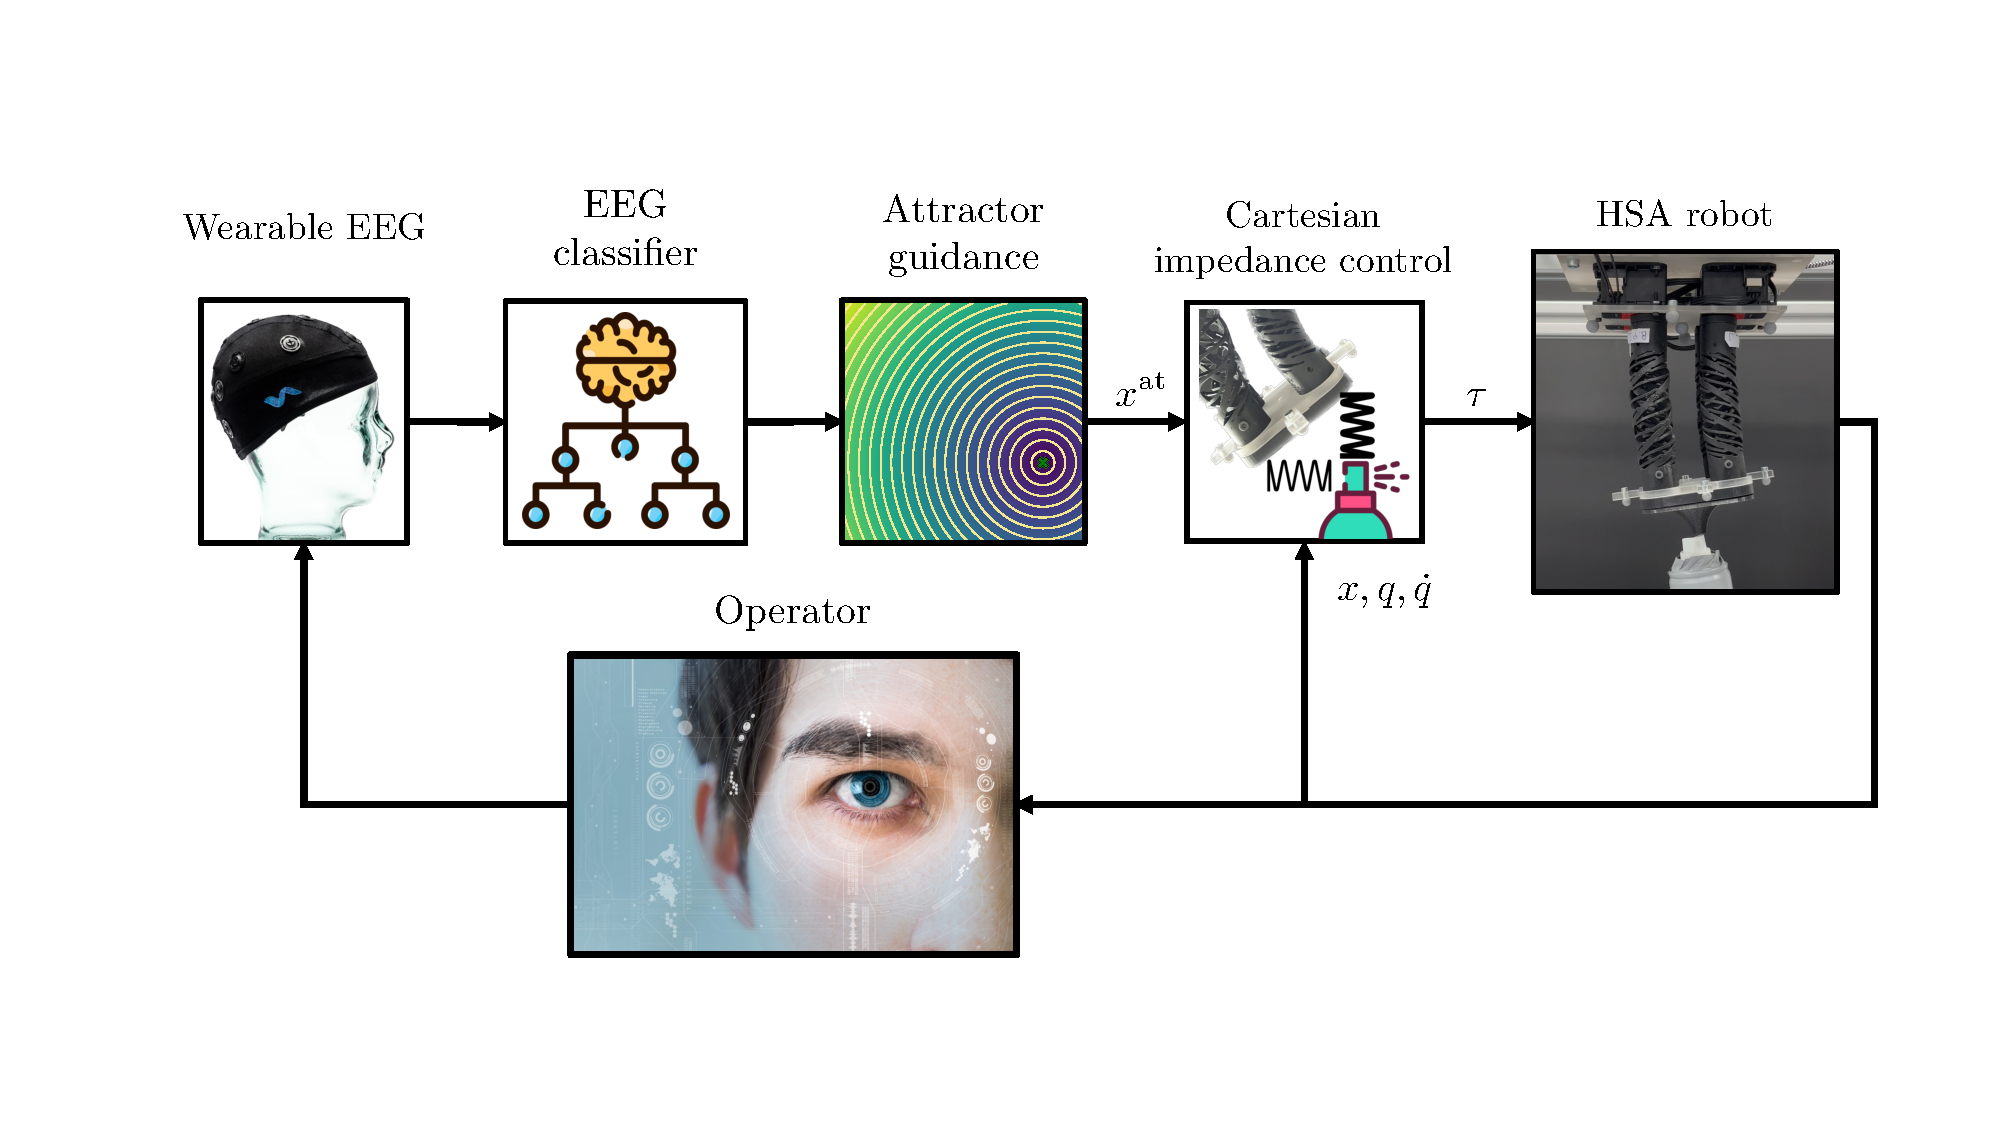
\includegraphics[width=0.7\columnwidth]{braincontrol/figures/control_scheme/control_scheme_high_level_overview_cropped.pdf}
    \caption{High-level control scheme of an operator steering an \gls{HSA} robot with brain signals. We leverage the \gls{EEG} signal classifications for guiding an attractor in the plane. Subsequently, an impedance controller is designed to shape the impedance in Cartesian space and render the attractor to be a globally asymptotically stable equilibrium of the potential.}
    \label{fig:braincontrol:control_scheme_high_level_overview}
\end{figure}

While \gls{BMI}-based assistance has been investigated with a focus on 
% exoskeletons~\citep{wairagkar2016movement, araujo2021development} 
soft exosuits assisting hand-rehabilitation ~\citep{zhang2019eeg} or with strenuous arm acitivites~\citep{tacca2022neuro}, 
% \textcolor{red}{TODO: insert combination of a) soft robotics and BCI are both emerging fields, b) most of the focus has been on binary decisions }
it is still an open challenge how \gls{BMI} can be used for controlling soft manipulators. 
%One key reason for existing strategies developed for soft exosuits and hands not being directly applicable to more complex soft robots is that those strategies restricted the interface to binary decisions such as \emph{open} / \emph{close}. To overcome these limitations, 
In this chapter, we make a first step towards solving this challenge by proposing a pipeline (see Fig. \ref{fig:braincontrol:control_scheme_high_level_overview}) that lets the user steer the soft robot's end-effector in Cartesian space. The two key ingredients are a novel mapping strategy transforming the brain signals into meaningful references and Cartesian impedance control. The latter is essential because it allows for preserving the robot's compliance in closed-loop \citep{della2017controlling}. We build the proposed \gls{BMI} pipeline around a \gls{HSA} soft robot \citep{stolzle2023modelling, stolzle2024experimental}, % truby2021recipe
which relies on architected metamaterials and electrical actuation to elongate, bend, and twist.
\gls{HSA} robots are an excellent match for our test case of assting with \gls{ADL}, as they can be portable because of their electrical actuation, they are compact and combine many \glspl{DOF} in one segment, and easy to manufactury via 3D printing~\citep{truby2021recipe}.
% This makes the control problem especially challenging because of the peculiarity of these systems' dynamics, namely underactuation and non-affinity in control. % We provide more details on innovation from the model-based control standpoint in Section~\ref{sub:braincontrol:computational_controller}.

\begin{figure}[hbt]
    \centering
    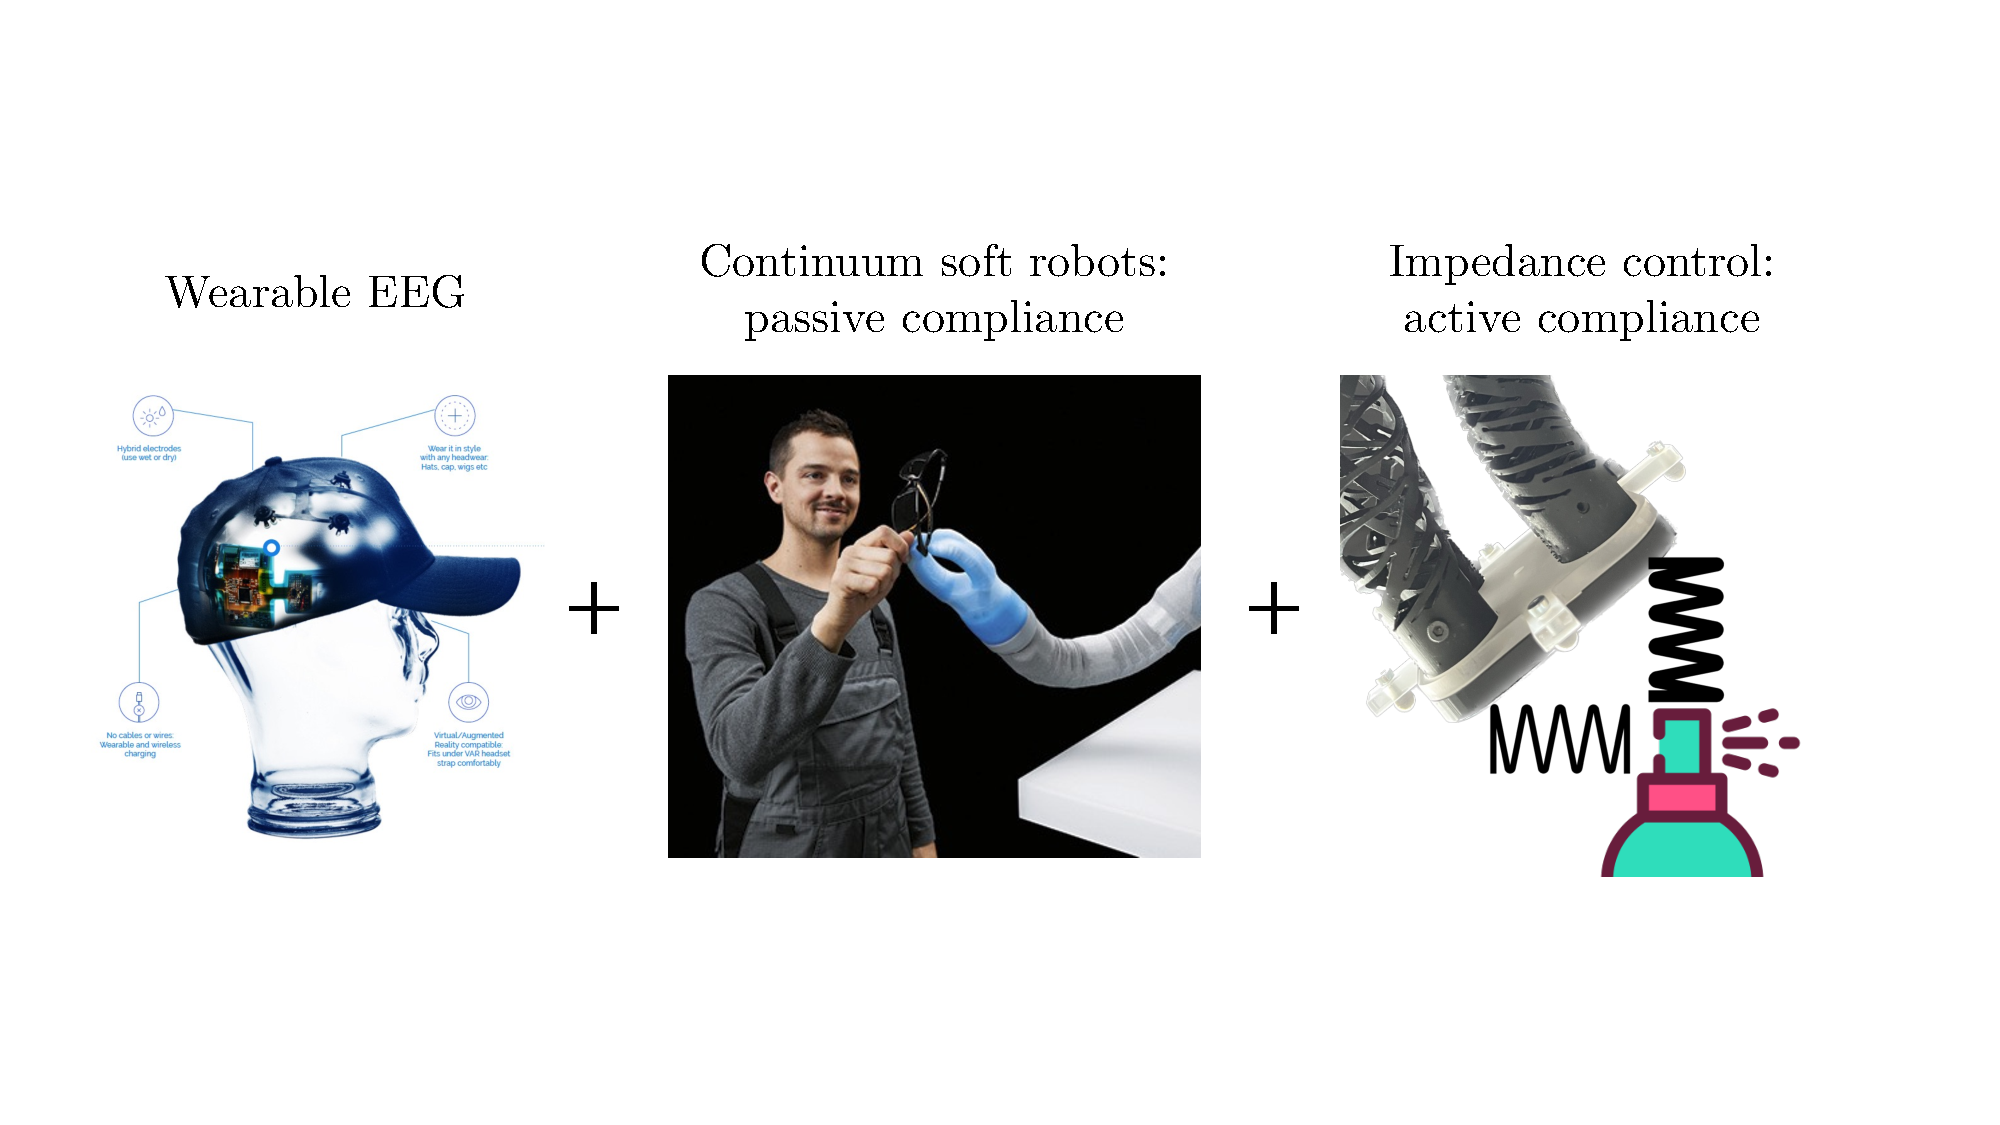
\includegraphics[width=0.7\textwidth]{braincontrol/figures/embodied_computational_intelligence/embodied_and_computational_intelligence_cropped.pdf}
    \caption{In this work we propose combining wearable \gls{EEG} devices with continuum soft robots and impedance control. The classification accuracy of motor imagery based on signals from few-channel, wearable \gls{EEG} devices is currently limited to less than \SI{75}{\percent}. The inevitable operation errors can be accepted by establishing both passive and active compliance: The embodied intelligence of soft robots guarantees safety during interactions with the environment which is complemented by an impedance controller that allows us to design the Cartesian stiffness and damping charateristics of the robot.}
    \label{fig:braincontrol:embodied_computational_intelligence}
\end{figure}
 
We quantitatively verify the entire approach on mind-controlled setpoint regulation involving tracking a reference consisting of nine-step functions and demonstrate the qualitative behavior when assisting with a simple daily living activity. 
% Furthermore, we compare the performance of our motor imagery-based control to approaches giving the computational controller access to the privileged information of setpoints, which can considered to be an upper bound on performance.
Furthermore, we compare the performance of our motor imagery-based control to an approache that can be considered an upper bound on performance: The control using keyboard inputs is a very effective and efficient \gls{HMI} strategy, but requires the user to always interact physically with a keyboard,
which is not always desirable or possible (e.g., for users with disabilities).
% and (b) giving the computational controller access to the privileged information of setpoints.
% This control strategy now allows us to define the stiffness of the closed-loop system in Cartesian space. We verify the controller on the task of pressing the button of a perfume, which requires high stiffness in the normal direction of the interaction and flexibility in the tangential direction, allowing the soft robots to adapt to the environment interaction with physical intelligence.

Our contribution is establishing a \gls{BMI} strategy for continuum soft robots. This strategy is supported by experiments in which we perform setpoint regulation with a planar \gls{HSA} robot and motor imagery, which we experimentally validated on a simple \gls{ADL} task involving environment interaction: the user needs to steer the end-effector towards the tip of a hairspray container, apply force for releasing the fluid, and finally let the robot retreat from the contact.          

A video attachment to this chapter including recordings of experimental results can be found on YouTube\footnote{\url{https://youtu.be/wZTOxBPZmPc}}.
Furthermore, we have open-sourced our code including the OpenVibe pipeline on GitHub\footnote{\url{https://github.com/tud-phi/sr-brain-control}}.
\section{Methodology}
In this chapter, we let the user steer with motor imaginary brain signals the Cartesian position $x \in \mathbb{R}^2$ of the end-effector (i.e., the platform) of a planar \gls{HSA} robot.
We realize this strategy by first classifying the motor imaginary signals into Cartesian-space movement directions (e.g., the active axis and sign of the movement). We use this information to adjust the position of a task-space attractor iteratively (see Section~\ref{sub:braincontrol:planning_attractors_switching}). % Section~\ref{sub:braincontrol:computational_controller} describes how a model-based computational controller establishes this attractor. Importantly, we preserve the soft robot's compliance by shaping the closed-loop system's impedance in Cartesian space.


\subsection{Background: Motor Imagery-based BMI systems}\label{sub:braincontrol:motor_imagery_bmi}

Imagining the movement of body parts or limbs (e.g., hands, legs, tongue) without moving it or the mental rehearsal of a motor act without overt movement execution is termed Motor Imagery~\cite{lotze2006motor}.  The neuronal activities observable inside a frequency range of \SI{8}{Hz} to \SI{12}{Hz} (Mu) and \SI{12}{Hz} to \SI{30}{Hz} (Beta) are associated with cortical areas directly connected to the brain’s motor output (activating primary sensorimotor areas that can be modulated with imaginary mental movement in healthy as well people with neuromuscular disabilities). 
% Motor Imagery is widely used for the BMI systems involved in either task-specific for instance exoskeleton /cite!!, or motion wheelchair /cite!!.

The motor imagery \gls{BMI} framework typically consists of four integral components:

\begin{enumerate}
    \item \textbf{Signal acquisition:} The initial stage involves the recording of neural signals while the person imagines the movements of the limbs, generally acquired using noninvasive methodologies (e.g., \gls{EEG}).
    \item \textbf{Feature extraction:} Following signal acquisition, signal processing techniques are applied to extract salient features from the neural patterns associated with specific cognitive processes or intentions.
    \item \textbf{Feature translation:} This translation phase interprets the user's cognitive intent, converting it into actionable instructions for external devices.
    \item \textbf{Device output:} The culmination of the \gls{BMI} process is the application of the interpreted commands to external devices. 
    % \glspl{BMI} can be employed in various applications, ranging from motor control tasks, such as wheelchair navigation, to text input and the orchestration of complex robotic exoskeletons.
\end{enumerate}

As detailed further in Sec.~\ref{sub:braincontrol:bmi_protocol}, we leverage the difference in signals when imagining motor actions vs. rest state to control the sign of movement. The active axis of movement can be switched by clenching the jaw. % More details about the \gls{BMI} protocol can be found in Section .
% To demonstrate the proof of concept, in our work, we focus on Motor Imagery imagination v/s rest state which is used as a control, further described in Section \ref{sub:braincontrol:bmi_protocol}

% \subsection{Planning attractors with brain signals (multi-class)}\label{sub:braincontrol:planning_attractors_multiclass}
% We classify the \gls{EEG} signals into \textcolor{orange}{four classes: move left ($u=(1, 0)$), move right ($u=(-1, 0)$), move down ($u=(0, 1)$), and move up ($u=(0, -1)$)}. More details about the procedure used to process and classify \gls{EEG} signals can be found in Section~\ref{ssub:braincontrol:eeg_pipeline}.
% Subsequently, this information is used to manipulate an attractor position $x^\mathrm{at} \in \mathbb{R}^2$, which is later tracked by a computational controller (see Section~\ref{sub:braincontrol:computational_controller}). The following policy is used to update the attractor at each time step $k$:
% \begin{equation}
%     x^\mathrm{at}(k) = x^\mathrm{at}(k-1) + \Delta_\mathrm{x} \, u(k),
% \end{equation}
% where $\Delta_\mathrm{x}$ is a tunable constant influencing the velocity of the attractor.

\subsection{Planning attractors with brain signals}\label{sub:braincontrol:planning_attractors_switching}
Our brain signal processing pipeline provides us with two pieces of information at each time step $k$: i) the unit vector $e_\mathrm{a}(k) \in \{ [1, 0]^\mathrm{T}, [0, 1]^\mathrm{T} \}$ corresponding to the current active axis of movement % with $\lVert e^\mathrm{at} \rVert = 1$
and ii) the sign of movement $s(k) \in \{ -1, 1 \}$. We use $e_\mathrm{a}(k)$ and $s(k)$ to incrementally steer a virtual attractor defined in operational space $x^\mathrm{at} \in \mathbb{R}^2$ as follows
%
%The following policy is used to update the attractor at each time step $k$:
\begin{equation}
    u(k) = s(k) \, e_\mathrm{a}(k) \in \mathbb{R}^2, \quad  x^\mathrm{at}(k) = x^\mathrm{at}(k-1) + \Delta_\mathrm{x} \, u(k),
\end{equation}
where $\Delta_\mathrm{x} \in \mathbb{R}^+$ is a tunable constant influencing the velocity of the attractor movement.
%
Later, we will shape the potential field with a computational controller such that the attractor becomes a globally asymptotically stable equilibrium (see Section~\ref{sub:braincontrol:computational_controller}).

\begin{figure}
\begin{center}
    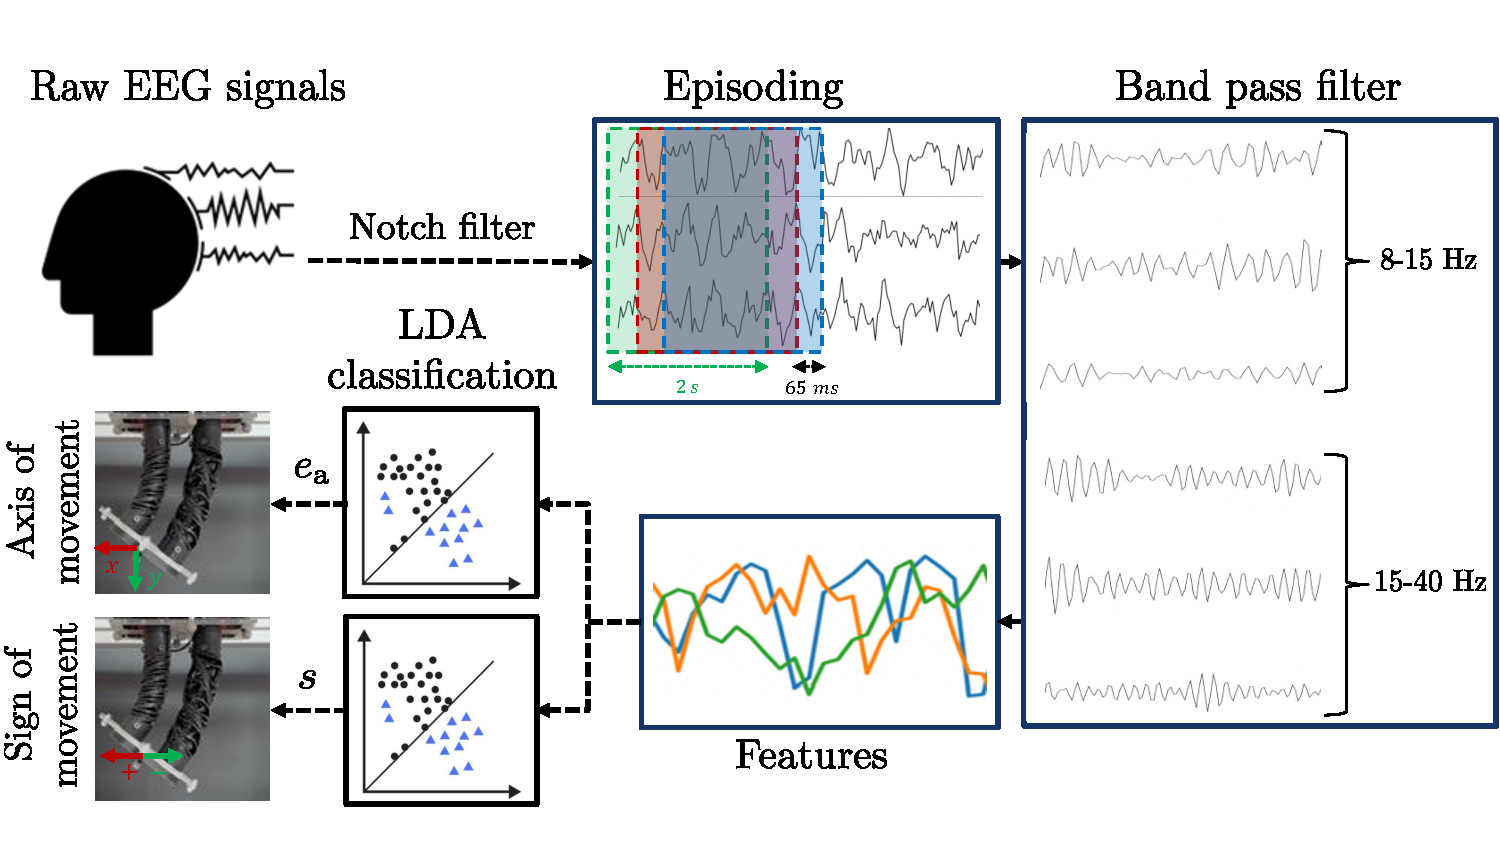
\includegraphics[width=\columnwidth]{braincontrol/figures/eeg_pipeline/eeg_pipeline_v3_compressed.pdf}
    \caption{EEG data processing pipeline: The EEG data is acquired in real-time, pre-processed, and divided into episodes and subbands. Next, we extract power features and pass them to two LDA classifiers: the first outputs the axis of movement (for example, moving along the x- or y-axis), and the second provides the sign of movement (for example, positive or negative movement along the active axis). These commands are then used to move the attractor in Cartesian space.}
    \label{fig:braincontrol:eeg_pipeline}
\end{center}
\end{figure}

\subsection{Computational controller}\label{sub:braincontrol:computational_controller}
We adopt the Cartesian impedance controller from \textcolor{red}{Sec.~\ref{sub}} to shape the potential field with a computational controller such that the attractor $x^\mathrm{at}$ becomes a globally asymptotically stable equilibrium
\begin{equation}\label{eq:braincontrol:cartesian_impedance_controller}
\begin{split}
    \tau =& \: J^\mathrm{T}(q) \, \left (K_x \, (x^\mathrm{at} - x) - D_x \, \dot{x} \right ) + G(q) + K \, (q-q^0)\\
    & \: + J^\mathrm{T}(q) \, J_\mathrm{B}^{+\mathrm{T}}(q) \, D \, \dot{q} + J^\mathrm{T}(q) \, \mu(q,\dot{q}) \left ( I_3 - J_\mathrm{B}^+(q) J(q) \right )\dot{q}.
\end{split}
\end{equation}

% \begin{figure}
%     \centering
%     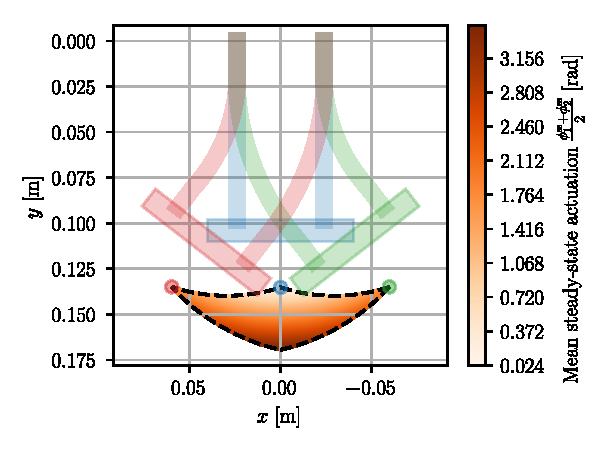
\includegraphics[width=0.85\columnwidth, trim={10 10 10 10}]{braincontrol/figures/workspace/operational_workspace_fpu_with_ee.pdf}
%     \caption{Operational workspace of a HSA robot with attached end-effector: the color displays the mean steady-state actuation $\frac{\phi_1^\mathrm{ss} + \phi_2^\mathrm{ss}}{2}$ necessary for the end-effector to remain at the position. Additionally, we visualize three example shapes: the straight configuration with $\phi^\mathrm{ss} = (0, 0)$ (blue), maximum clockwise bending with $\phi^\mathrm{ss} = (3.49, 0) \, \si{rad}$ (red), and maximum counter-clockwise bending with $\phi^\mathrm{ss} = (0, 3.49) \, \si{rad}$ (green).}
%     \label{fig:braincontrol:hsa_workspace}
% \end{figure}

\begin{figure*}
\begin{center}
    \subfigure[Operational workspace]{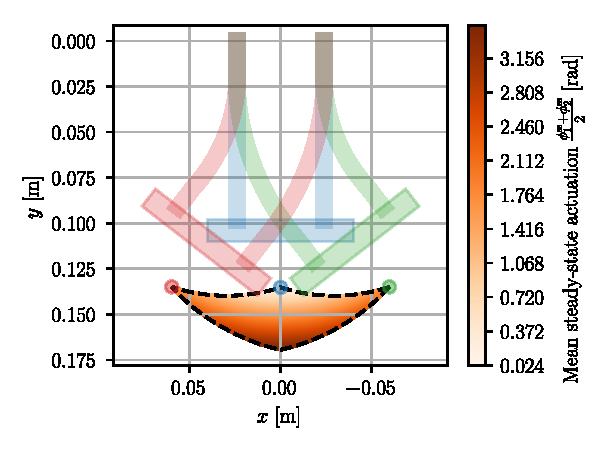
\includegraphics[width=0.36\linewidth]{braincontrol/figures/workspace/operational_workspace_fpu_with_ee.pdf}\label{fig:braincontrol:hsa_workspace}}
    \subfigure[Experimental setup]{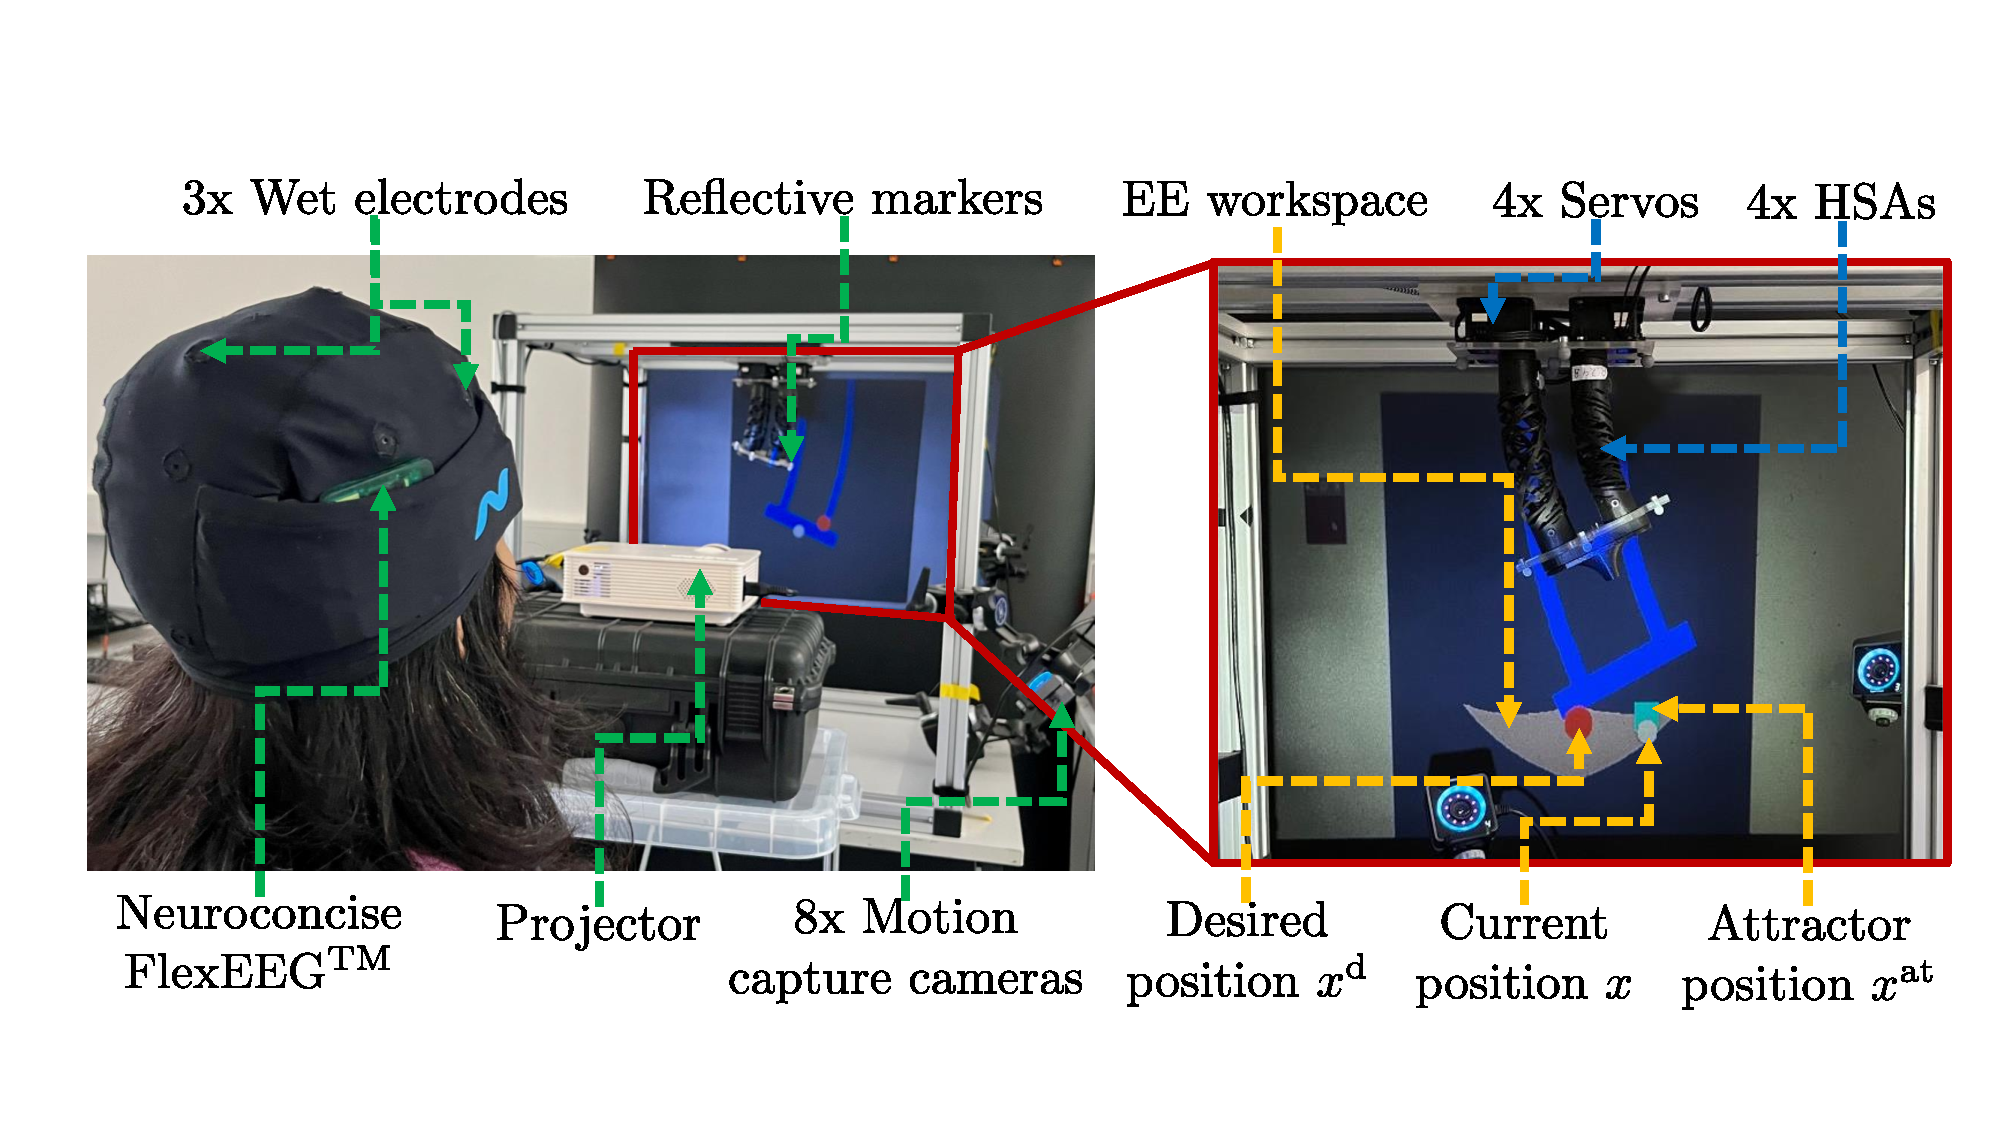
\includegraphics[width=0.63\linewidth]{braincontrol/figures/experimental_setup/experimental_setup_v3_cropped.pdf}\label{fig:braincontrol:experimental_setup}}
    \caption{\textbf{Panel (a:} Operational workspace of a HSA robot with attached end-effector: the color displays the mean steady-state actuation $\frac{\phi_1^\mathrm{ss} + \phi_2^\mathrm{ss}}{2}$ necessary for the end-effector to remain at the position. Additionally, we visualize three example shapes: the straight configuration with $\phi^\mathrm{ss} = (0, 0)$ (blue), maximum clockwise bending with $\phi^\mathrm{ss} = (3.49, 0) \, \si{rad}$ (red), and maximum counter-clockwise bending with $\phi^\mathrm{ss} = (0, 3.49) \, \si{rad}$ (green).
    \textbf{Panel (b):} The HSA robot is mounted platform-down to a motion capture cage with 8x Optitrack PrimeX 13 cameras, which track the 3D pose of the platform (i.e., the end-effector). A Dynamixel MX-28 servo actuates each of the four HSAs. We project a rendering of the current (white dot) and desired (red dot) end-effector position, the attractor (green square), and the operational workspace (grey area) onto the black screen in the background. The study subject wears a cap with the Neuroconcise FlexEEG sensor, and we acquire the data of three electrodes connected to the motor cortex.}
\end{center}
\end{figure*}

\begin{figure}
\begin{center}
    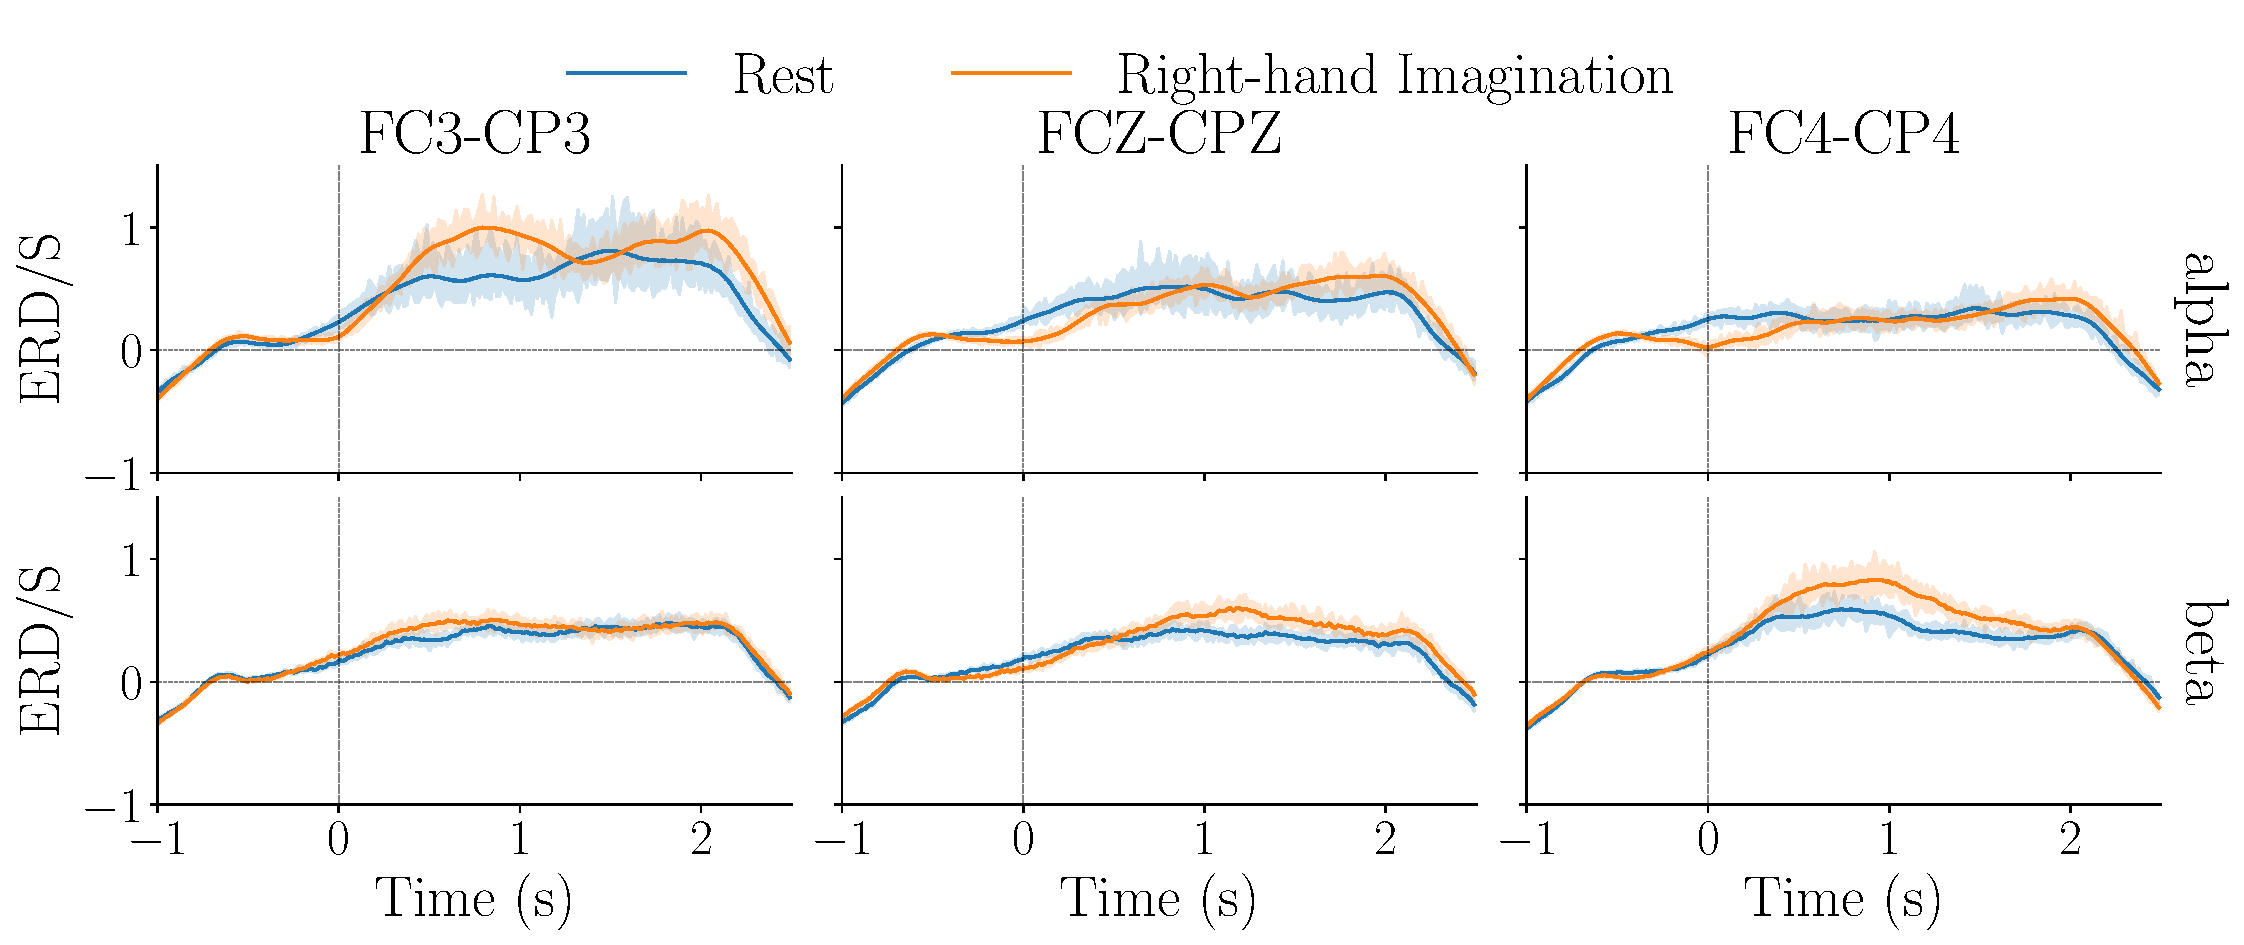
\includegraphics[width=0.85\columnwidth]{braincontrol/figures/eeg_pipeline/ERDS.pdf}
    \caption{ERD/S (overall average) over a time period of \SI{2.5}{s} of training data for right-hand Imagination v/s rest state including the Alpha and Beta bands of the EEG signals  where the cue is presented at \SI{0}{s}. We plot the data of three sensors (i.e., channels): FC3-CP3 (left), FCZ-CPZ (middle) and FC4-CP4 (right).}
    \label{fig:braincontrol:ERDS}
\end{center}
\end{figure}

\begin{figure*}[t]
    \centering
    \subfigure[End-effector x-coordinate]{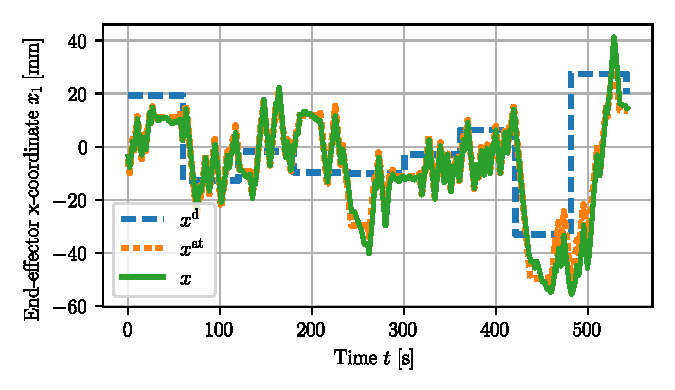
\includegraphics[width=0.47\textwidth, trim={5, 5, 5, 5}]{braincontrol/figures/setpoint_regulation/20231031_185546_pee_x.pdf}\label{fig:braincontrol:experimental_results:setpoint_regulation:brain:pee_x}}
    \subfigure[End-effector y-coordinate]{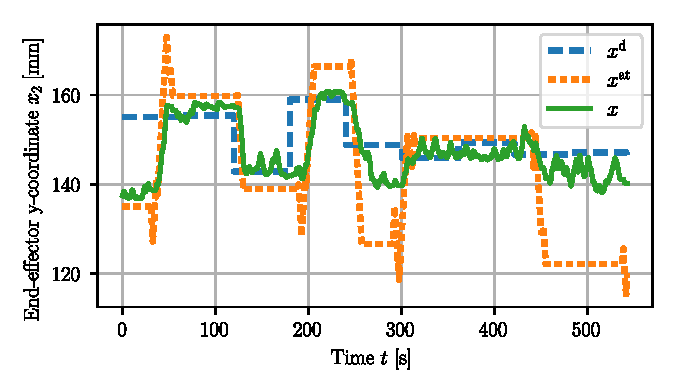
\includegraphics[width=0.47\textwidth, trim={5, 5, 5, 5}]{braincontrol/figures/setpoint_regulation/20231031_185546_pee_y.pdf}\label{fig:braincontrol:experimental_results:setpoint_regulation:brain:pee_y}}\\
    \subfigure[Configuration $q$]{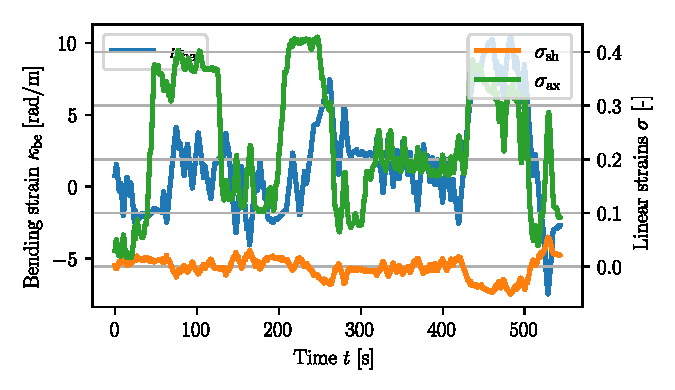
\includegraphics[width=0.47\textwidth, trim={5, 5, 5, 5}]{braincontrol/figures/setpoint_regulation/20231031_185546_q.pdf}\label{fig:braincontrol:experimental_results:setpoint_regulation:brain:q}}
    \subfigure[Control input $\phi$]{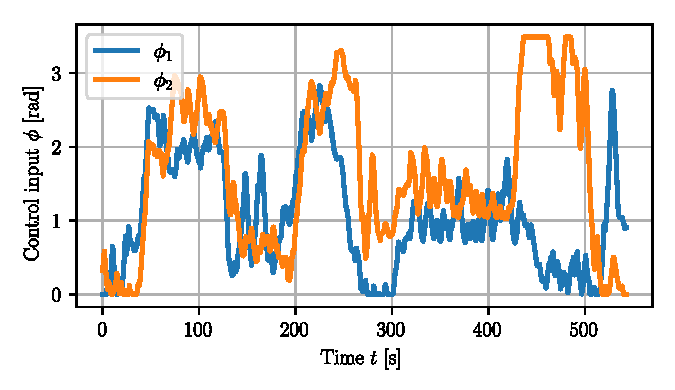
\includegraphics[width=0.47\textwidth, trim={5, 5, 5, 5}]{braincontrol/figures/setpoint_regulation/20231031_185546_phi.pdf}\label{fig:braincontrol:experimental_results:setpoint_regulation:brain:phi}}
    \caption{Experimental results for tracking a reference trajectory of nine step functions with motor imagery. \textbf{Panel (a) \& (b):} The x/y-coordinate of the end-effector position with the solid line denoting the actual position, the dotted line the attractor position, and the dashed line the reference (i.e., the setpoint).
    \textbf{Panel (c):} The evolution of the configuration.
    \textbf{Panel(d):} The saturated planar control inputs. }\label{fig:braincontrol:experimental_results:setpoint_regulation:brain}
\end{figure*}
\section{Experiments}

\subsection{Experimental setup}
In the following, we detail the \gls{EEG} data processing procedure (see also Fig.~\ref{fig:braincontrol:eeg_pipeline}) and present our experimental setup, which is annotated in Fig.~\ref{fig:braincontrol:experimental_setup}.

\subsubsection{EEG data processing}\label{ssub:braincontrol:eeg_pipeline}
We integrate the 3-channel flexEEG Neuroconcise device with the OpenVibe software
% through a Lab Streaming Layer (LSL) 
to acquire the EEG data and process it in real-time.
This configuration facilitates data recording and cue presentation. We process the \gls{EEG} signals at a sampling frequency of \SI{125}{Hz} with a pipeline that involves three bi-polar channels around the motor cortex: FC3-CP3, FCZ-CPZ, and FC4-CP4.
After a notch filter of \SI{50}{Hz}, we apply Independent Component Analysis (ICA) to extract three independent components from the recorded \gls{EEG} data, which is represented by the equation $S(t) = W \, X(t)$, where $S(t)$ are the extracted independent components and $W$ represents the unmixing matrix, allowing us to separate eye blink artifacts in \gls{EEG} signals, which is critical for enhancing the accuracy. 
Subsequently, we apply a Butterworth filter bank to isolate specific frequency bands of interest, including 8-15 \si{Hz} and 15-42 \si{Hz}. 
% removed because of space constraints
% The general equation for a Butterworth filter of order $N$ for a given frequency range (e.g., 8-15 \si{Hz}) is
% \begin{equation}
%     H(f) = \frac{1}{{1 + \left(\frac{f}{f_\mathrm{c}}\right)^{2N}}},
% \end{equation}
% where $H(f)$ represents the frequency response of the filter, $f$ is the frequency of the \gls{EEG} signal, $N$ is the filter order, and $f_\mathrm{c}$ is the critical frequency (i.e., center frequency) of the desired frequency band.
This enhances the ability to analyze \gls{EEG} data by isolating and examining different frequency band components within the \gls{EEG} signals. Once the signals are filtered in sub-bands and epoched with a duration of \SI{2}{s} and time interval of \SI{0.065}{s}, the features are extracted by the log of the power: $L_i(t) = \log\left(P_i(t)\right)$, where the power $P_i(t) = |E_i(t)|^2$ is represented by square of magnitude of the \gls{EEG} signal $E_i(t)$ at time instance $t$.
These features are then provided to a classifier, which we select as \gls{LDA} due to its simplicity~\citep{lotte2014tutorial}.

We implement a second classifier with the same pipeline, where jaw clenching is provided as a muscle artifact that is classified v/s raw EEG data. 
\subsubsection{Robotic system}
% HSA robot
We consider a robot consisting of four \gls{HSA} rods, which were 3D printed via digital projection lithography % ~\citep{truby2021recipe} 
from the photopolymer resin Carbon FPU 50. % ~\citep{carbon:fpu50}.
Each \gls{HSA} rod is electrically actuated by a Dynamixel M-28 servo up to a maximum twist angle of $\phi_\mathrm{max} = \SI{3.49}{rad}$.
% MoCap
The robot is attached platform-down to a motion capture cage with eight Optitrack Prime X13 cameras tracking at \SI{200}{Hz} the pose of reflective markers attached to the end-effector of the \gls{HSA} robot.
We estimate the current Cartesian-space velocity of the end-effector with a Savitzky-Golay filter. 
Subsequently, we leverage a closed-form expression of the inverse kinematics of a \gls{CS} model~\citep{stolzle2024experimental} to compute the current configuration $q$ of the robot.
% projector
We render an image of the current shape of the robot together with the present end-effector position (white dot), the attractor planned by the user (green square), the operational workspace (grey, see also Fig.~\ref{fig:braincontrol:hsa_workspace}) and if applicable, the goal position (red dot). 
We specify the currently active axis of movement $e_\mathrm{a}$ with a double arrow and project the resulting image onto a black screen in the background of the motion capture cage.
% control/software architecture
The robot is operated with a ROS2 software framework\footnote{\url{https://github.com/tud-phi/ros2-hsa}}. We receive the predicted and classified brain signals via TCP at a frequency of \SI{18}{Hz} and move the attractor subsequently with $\Delta_\mathrm{x} = \SI{0.2}{mm}$. We evaluate the Cartesian impedance controller using the gains $K_\mathrm{p} = \SI{300}{N \per m}$, $K_\mathrm{d} = \SI{1.5}{N s \per \meter}$ at a frequency of \SI{50}{Hz} and finally send the desired motor positions to the servos.

% latency computation
% FlexEEG device
% For 24bit and 250 Hz, the time between packets is 47ms.
% transit time between FlexEEG and pc is ~35ms
% OpenVibe data processing and classification
% running at 125Hz, so maximum latency of 8ms
% joylike operation
% queries the TCP connection at 100Hz, therefore maximum delay of 10ms
% computational control loop
% runs at 50Hz, so maximum delay of 20ms
% communication with dynamixel motors
% dual-way communication works at 100Hz, so maximum delay (solely based on communication) of 10ms
The entire control pipeline from measuring \gls{EEG} signals to sending the actuation commands to the motors exhibits a maximum latency of (i.e., is upper-bounded by)  \SI{130}{ms}.

\subsection{BMI protocol}\label{sub:braincontrol:bmi_protocol}
In the following, we will describe the protocol for collecting the motor imagery dataset, training the \gls{EEG} classifiers, and mapping classifier outputs into actionable robot commands.

\subsubsection{Training protocol}

The participant is given brief instructions about motor imagery signals.
We follow the Graz-BCI~\citep{roc2021review} paradigm, which assists with training, where the display of the cue instructs the participant to perform imagination of movements: when a left arrow appears, the participant is asked to rest and not focus on motor movement. When the right arrow appears on the screen, the participant is asked to imagine the motor activity from the dominant hand (here, the right hand), such as grasping or squeezing an object. The training protocol for right-hand motor imagery v/s rest demands fifty cues per class. 
We similarly collect data for the second classifier by asking participants to clench their jaw, which can be detected as muscular artifacts (vs. no muscular movement) in the \gls{EEG} signals.
At the end of the trial, we train both classifiers (see Sections~\ref{sub:braincontrol:motor_imagery_bmi} and \ref{ssub:braincontrol:eeg_pipeline} for more information) and repeat the procedure until an accuracy of \SI{75}{\percent} is obtained for right-hand motor imagery v/s rest and accuracy of \SI{85}{\percent} for jaw clench artifact v/s raw EEG.
We evaluate the trained motor imagery classifier on the test set and report the results in Tab.~\ref{tab:braincontrol:confusion_matrix}.

\begin{table}[hbt]
    \centering
    \begin{tabular}{c c|c c}
        %  \toprule
        & & \multicolumn{2}{c}{\textbf{Prediction}}\\
        \rule{0pt}{4ex} && Rest & \makecell{Right-handed\\ motor imagery} \\
        \midrule
        & Rest & \SI{70.7}{\percent} & \SI{29.3}{\percent}\\
        \raisebox{\dimexpr 2ex}[0pt][0pt]{\rotatebox[origin=c]{90}{\small \textbf{Label}}} & \makecell{Right-handed\\ motor imagery} & \SI{33.3}{\percent} & \SI{68.7}{\percent}\\
         % \bottomrule
    \end{tabular}
    \caption{Confusion matrix for the \gls{LDA} classifier at predicting right-hand motor imagery vs. rest based on the preprocessed \gls{EEG} signals evaluated on a test set.}
    \label{tab:braincontrol:confusion_matrix}
\end{table}

% \definecolor{adaee4ed-88c8-5b21-a9e7-31316ebef86f}{RGB}{255, 179, 178}
% \definecolor{f3551e38-74df-57e2-b793-83d7fe876c85}{RGB}{0, 0, 0}
% \definecolor{0b71a967-1f15-55a5-9bb9-70efa7b4fc58}{RGB}{51, 51, 51}
% \definecolor{58712c6c-1b6d-5716-9834-102aad6341dc}{RGB}{175, 179, 255}
% \definecolor{70af333d-4869-5f2a-97ca-9904a9fce6c3}{RGB}{179, 254, 174}
% \definecolor{747aec21-333b-59ee-84e3-ddff893e5ccd}{RGB}{255, 216, 176}
% \definecolor{5856d031-3da1-575c-834e-c77e9e438c62}{RGB}{162, 177, 195}
% \tikzstyle{512bdd77-c3aa-5669-a956-85f7a90c6fb4} = [rectangle, rounded corners, minimum width=3cm, minimum height=1cm, text centered, font=\normalsize, color=0b71a967-1f15-55a5-9bb9-70efa7b4fc58, draw=f3551e38-74df-57e2-b793-83d7fe876c85, line width=1, fill=adaee4ed-88c8-5b21-a9e7-31316ebef86f]
% \tikzstyle{7f27e395-8473-5b8a-b568-31425bce482a} = [trapezium, trapezium left angle=70, trapezium right angle=110, minimum width=3cm, minimum height=1cm, text centered, font=\normalsize, color=0b71a967-1f15-55a5-9bb9-70efa7b4fc58, draw=f3551e38-74df-57e2-b793-83d7fe876c85, line width=1, fill=58712c6c-1b6d-5716-9834-102aad6341dc]
% \tikzstyle{e78ae073-3d46-5489-8262-483c8269c0e6} = [diamond, minimum width=3cm, minimum height=2cm, text centered, font=\normalsize, color=0b71a967-1f15-55a5-9bb9-70efa7b4fc58, draw=f3551e38-74df-57e2-b793-83d7fe876c85, line width=1, fill=70af333d-4869-5f2a-97ca-9904a9fce6c3]
% \tikzstyle{69bbb168-da59-5865-902f-94e77902bf95} = [rectangle, minimum width=3cm, minimum height=1cm, text centered, font=\normalsize, color=0b71a967-1f15-55a5-9bb9-70efa7b4fc58, draw=f3551e38-74df-57e2-b793-83d7fe876c85, line width=1, fill=747aec21-333b-59ee-84e3-ddff893e5ccd]
% \tikzstyle{7be24b85-97d0-5b76-ba9e-d94005dca8f2} = [thick, draw=5856d031-3da1-575c-834e-c77e9e438c62, line width=2, ->, >=stealth]

% \begin{center}
% \begin{tikzpicture}[node distance=2cm]
% \node (start) [start] {Start};
% \node (training) [training, below of=start] {Training (no feedback)};
% \node (testing) [testing, below of=training] {Testing (with feedback)};
% \node (decision) [decision, below of=testing, yshift=-0.5cm] {Accuracy \textgreater 65?};
% \node (action) [action, below of=decision, yshift=-0.5cm] {HSA control real time};
% \draw [arrow] (start) -- (training);
% \draw [arrow] (training) -- (testing);
% \draw [arrow] (testing) -- (decision);
% %\draw [arrow] (training) -- (decision);
% \draw [arrow] (decision) -- node[anchor=east] {Yes} (action);
% \draw [arrow] (decision.east) -| ++(0.8,0.8) node[above right] {No} |- (testing.east);
% \label{Flowchart}
% \end{tikzpicture}
% \end{center}
% \begin{minipage}{\linewidth} 
% \captionsetup{justification=centering, singlelinecheck=false}
% \captionof{figure}{Protocol design of the Real-time HSA robots control}
% \end{minipage} 

\begin{figure}[t]
    \centering
    \subfigure[End-effector x-coordinate]{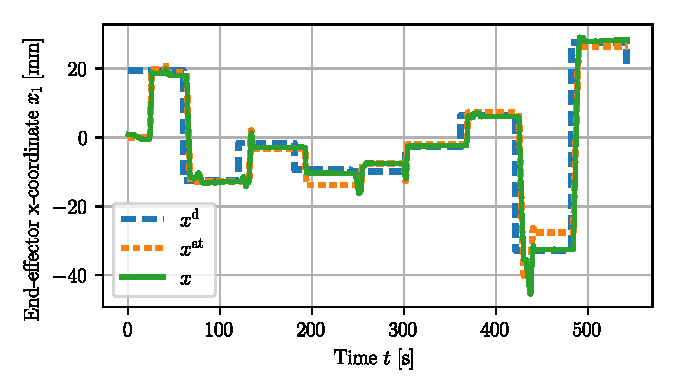
\includegraphics[width=0.47\textwidth, trim={5, 5, 5, 5}]{braincontrol/figures/setpoint_regulation/20231031_181745_pee_x.pdf}\label{fig:braincontrol:experimental_results:setpoint_regulation:keyboard:pee_x}}
    \subfigure[End-effector y-coordinate]{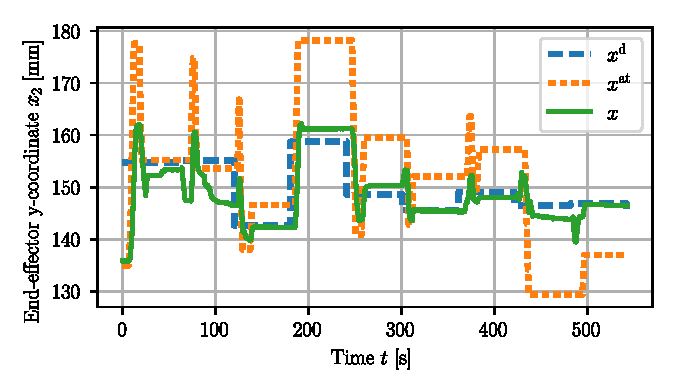
\includegraphics[width=0.47\textwidth, trim={5, 5, 5, 5}]{braincontrol/figures/setpoint_regulation/20231031_181745_pee_y.pdf}\label{fig:braincontrol:experimental_results:setpoint_regulation:keyboard:pee_y}}\\
    \subfigure[Configuration $q$]{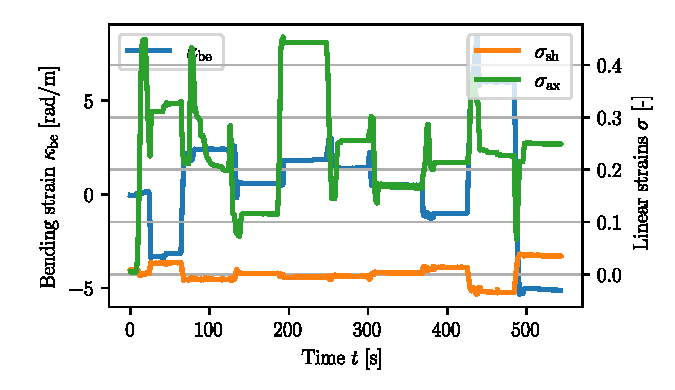
\includegraphics[width=0.47\textwidth, trim={5, 5, 5, 5}]{braincontrol/figures/setpoint_regulation/20231031_181745_q.pdf}\label{fig:braincontrol:experimental_results:setpoint_regulation:keyboard:q}}
    \subfigure[Control input $\phi$]{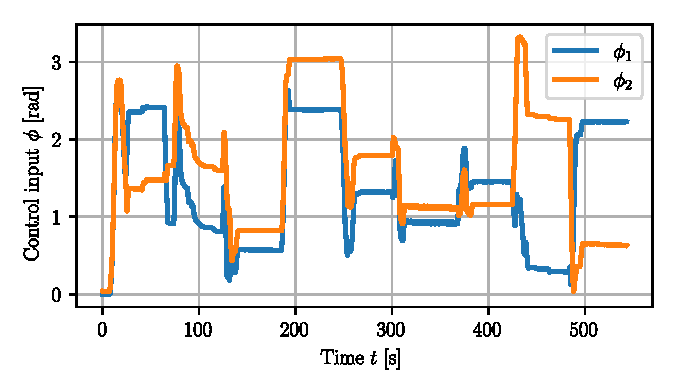
\includegraphics[width=0.47\textwidth, trim={5, 5, 5, 5}]{braincontrol/figures/setpoint_regulation/20231031_181745_phi.pdf}\label{fig:braincontrol:experimental_results:setpoint_regulation:keyboard:phi}}
    \caption{Experimental results for tracking a reference trajectory of nine step functions with keyboard inputs. \textbf{Panel (a) \& (b):} The x/y-coordinate of the end-effector position with the solid line denoting the actual position, the dotted line the attractor position, and the dashed line the reference (i.e., the setpoint).
    \textbf{Panel (c):} The evolution of the configuration.
    \textbf{Panel(d):} The saturated planar control inputs. }\label{fig:braincontrol:experimental_results:setpoint_regulation:keyboard}
\end{figure}




\subsubsection{Online robot control}
Now, the participant operates the HSA robot in real-time, with both classifiers being executed online.
Moreover, we map the outputs of the classifier into actionable commands: we initialize the x-axis as the active axis of movement (i.e., $e_\mathrm{a} = [1,0]$). When the first classifier detects jaw clenching for at least \SI{80}{\percent} of samples over a duration of \SI{2.8}{s}, we switch to the y-axis: $e_\mathrm{a} = [0,1]$ and vice-versa. If we do not detect any jaw-clenching artifacts, we evaluate the output of the second classifier in parallel: if there is motor imagery activity identified in the \gls{EEG} classifier, the attractor will be moved in the positive direction (i.e., $s=1$) along $e_\mathrm{a}$. In contrast, if the \gls{EEG} signals are classified as the participant being at rest, $s=-1$ (i.e., movement in the negative direction).

% ~\footnote{\url{https://www.neuroconcise.co.uk/}}.

\subsection{Setpoint regulation}\label{sub:braincontrol:experiments:setpoint_regulation}
We randomly generate nine setpoints $x^\mathrm{d}(t) \in \mathbb{R}^2$ within the operational workspace of the robot (see Fig.~\ref{fig:braincontrol:hsa_workspace} and display them as a red circle to the user over a duration of \SI{540}{s}.
The user can freely move the attractor to reach and keep the end-effector at the setpoint.
In addition to the motor imagery-based control, we conduct experiments where the subject controls the robot with a keyboard.
As a keyboard is a very efficient and precise \gls{HMI}~\citep{vasiljevic2016case, mahmud2020interface}, this represents an upper bound on the performance we could expect from the \gls{BCI}.
Here, the space button is used to switch that axis of movement $e_\mathrm{a}$ and positive/negative movement can be controlled via the left/right arrows.
% Furthermore, we execute an experiment in which the computational controller has access to normally privileged information: as we substitute $x^\mathrm{at}$ with $x^\mathrm{d}$ in \eqref{eq:braincontrol:cartesian_impedance_controller}, the Cartesian impedance controller now immediately regulates the robot towards the setpoint. By excluding the \gls{BMI} from the pipeline, this provides us with a reference of the performance we can expect from the computational controller and, with that, also represents a performance upper bound.

% sequence of stills with 10 images
\begin{figure*}[tb]
    \centering
    \subfigure[$t=\SI{0}{s}$]{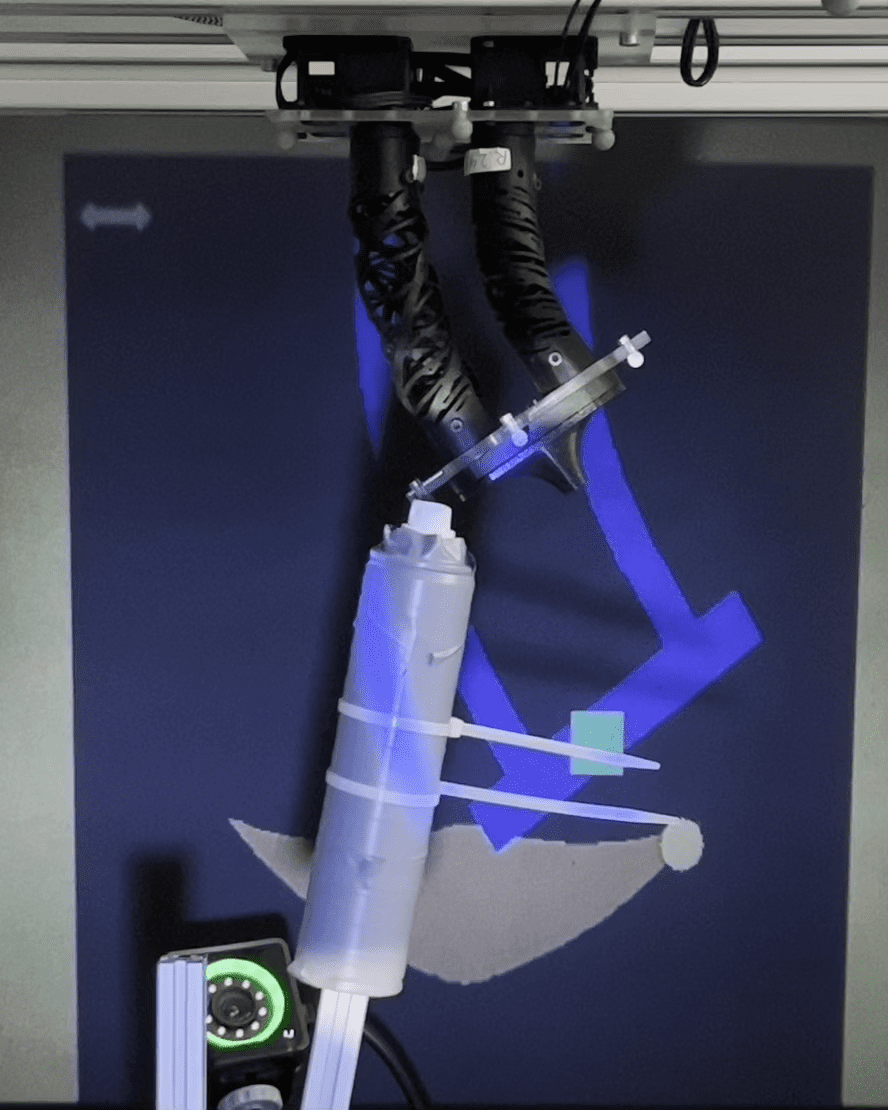
\includegraphics[width=0.192\textwidth]{braincontrol/figures/adl_task/20231031_203004_trimmed_and_cropped-0001-min.png}}
    \subfigure[$t=\SI{12}{s}$]{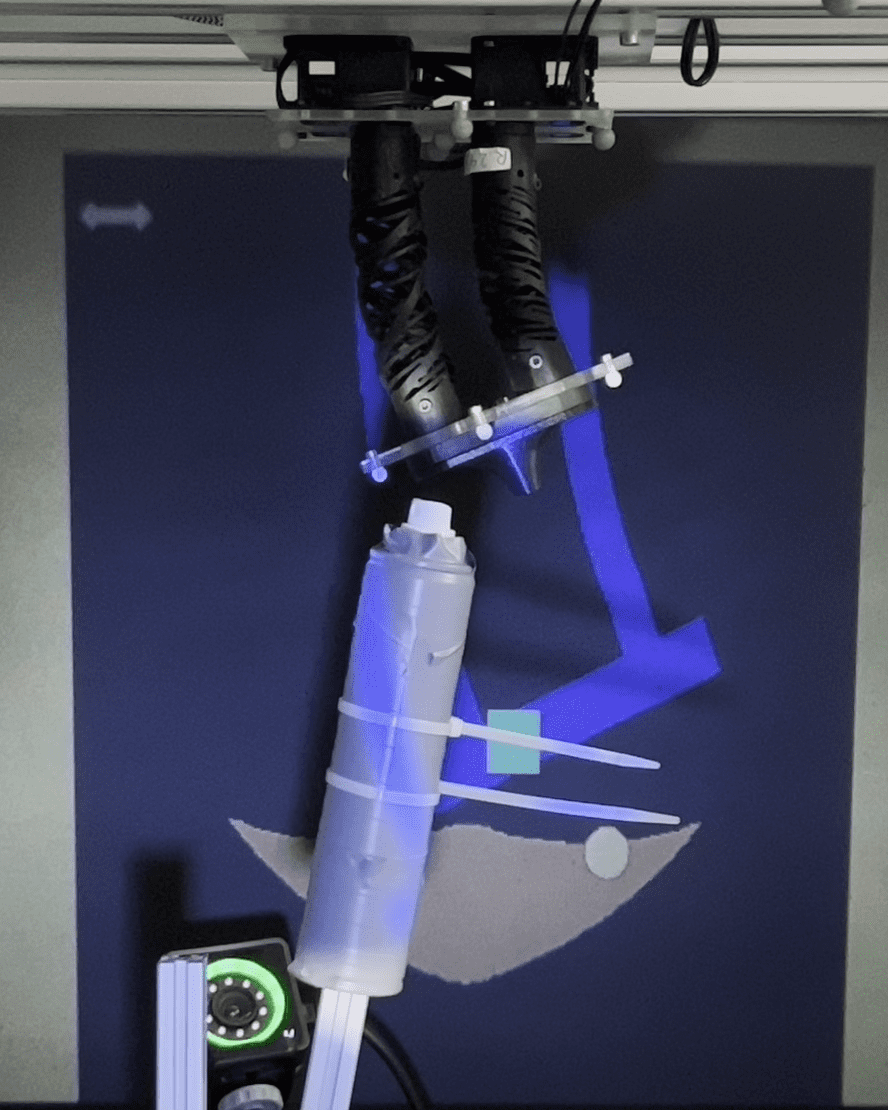
\includegraphics[width=0.192\textwidth]{braincontrol/figures/adl_task/20231031_203004_trimmed_and_cropped-0002-min.png}}
    \subfigure[$t=\SI{24}{s}$]{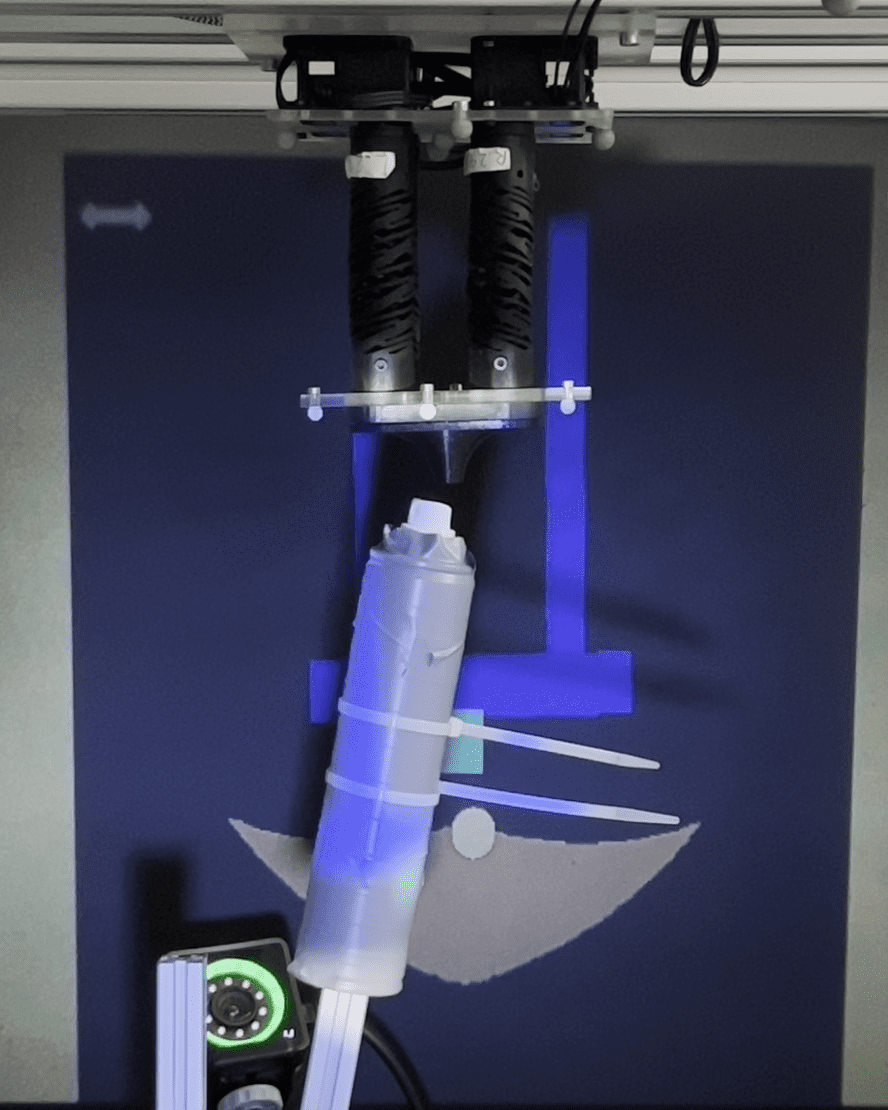
\includegraphics[width=0.192\textwidth]{braincontrol/figures/adl_task/20231031_203004_trimmed_and_cropped-0003-min.png}}
    \subfigure[$t=\SI{36}{s}$]{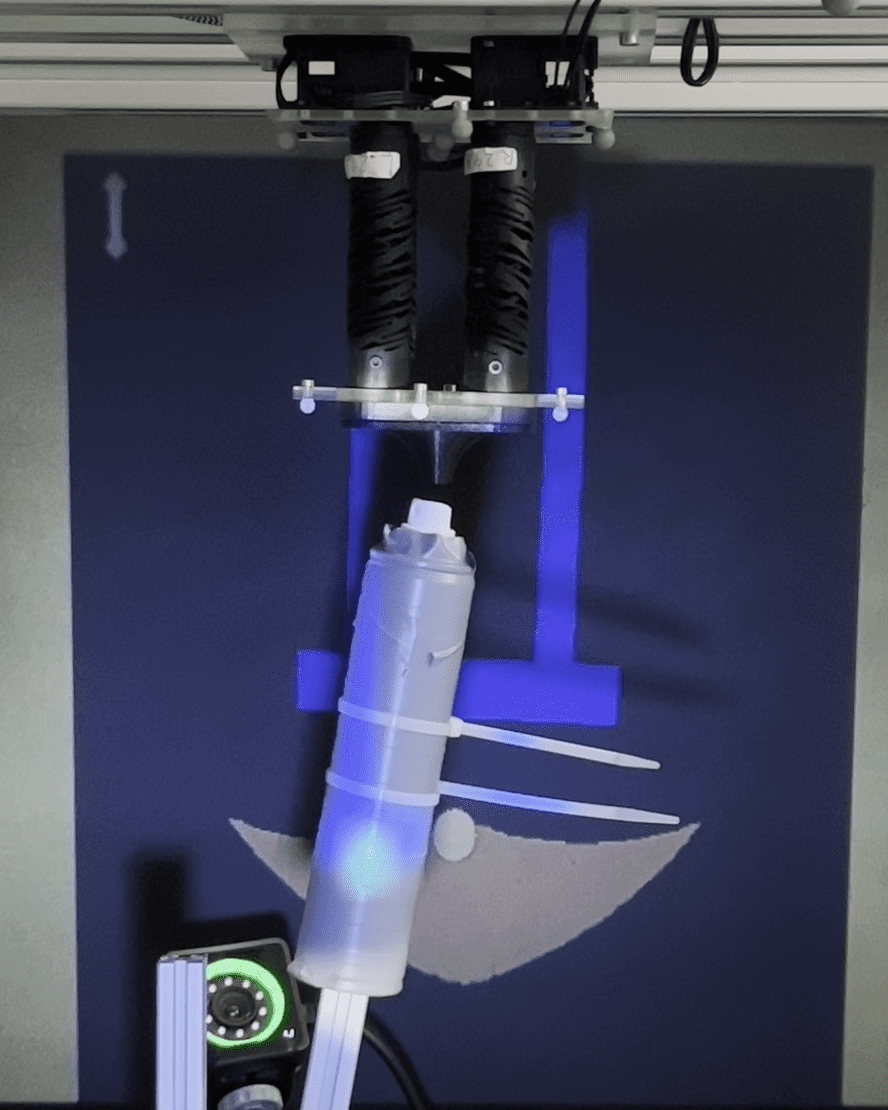
\includegraphics[width=0.192\textwidth]{braincontrol/figures/adl_task/20231031_203004_trimmed_and_cropped-0004-min.png}}
    \subfigure[$t=\SI{48}{s}$]{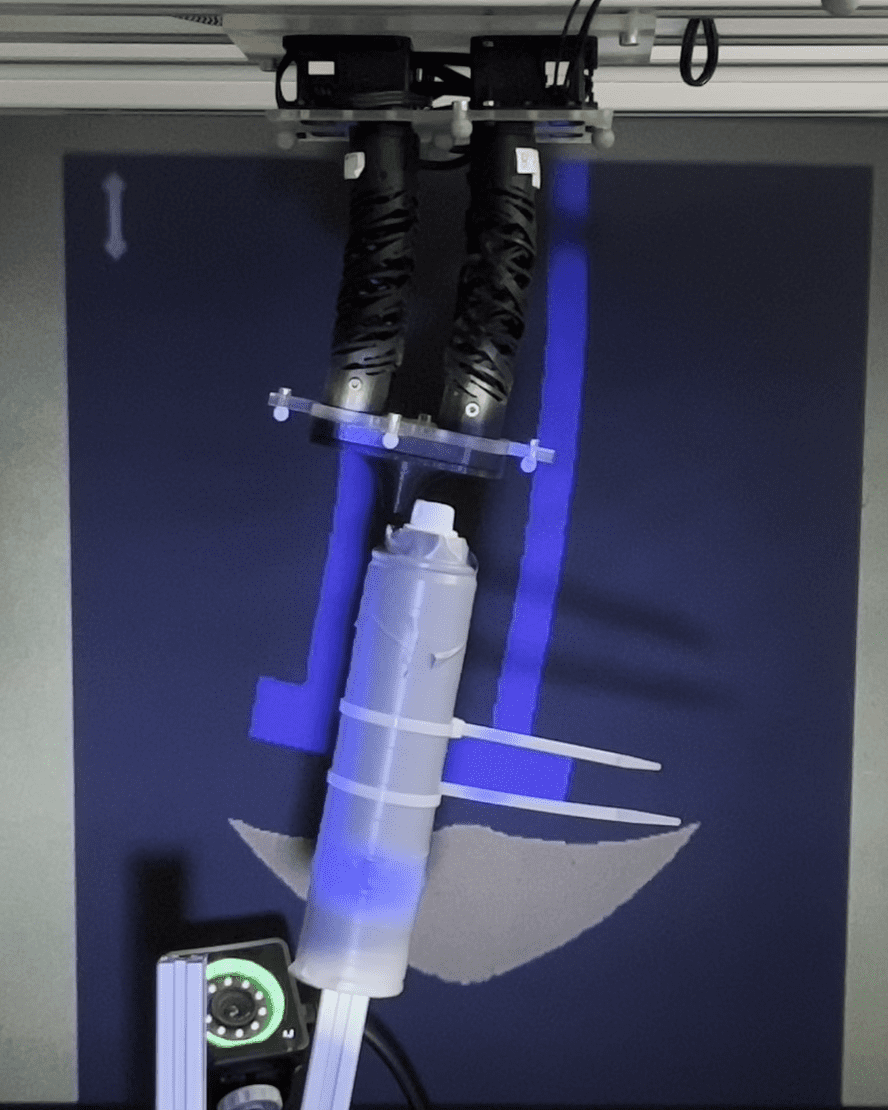
\includegraphics[width=0.192\textwidth]{braincontrol/figures/adl_task/20231031_203004_trimmed_and_cropped-0005-min.png}}\\
    \subfigure[$t=\SI{60}{s}$]{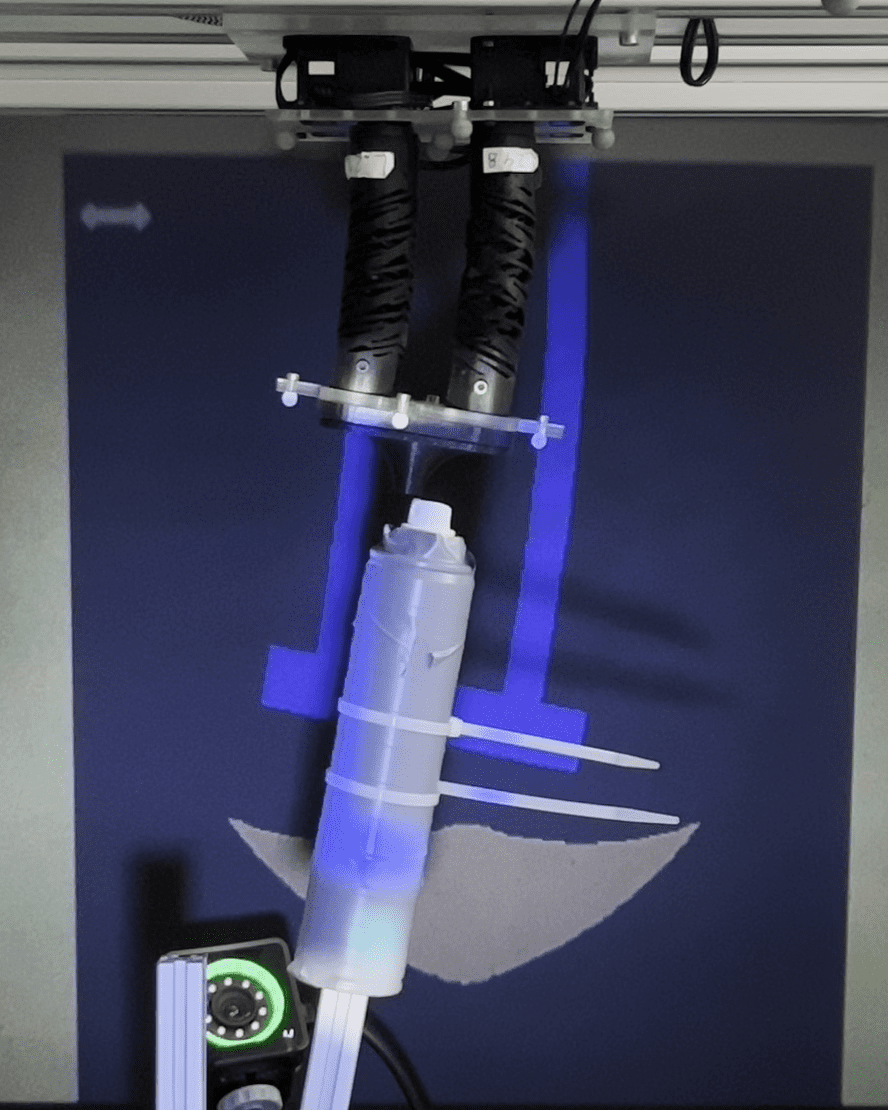
\includegraphics[width=0.192\textwidth]{braincontrol/figures/adl_task/20231031_203004_trimmed_and_cropped-0006-min.png}}
    \subfigure[$t=\SI{72}{s}$]{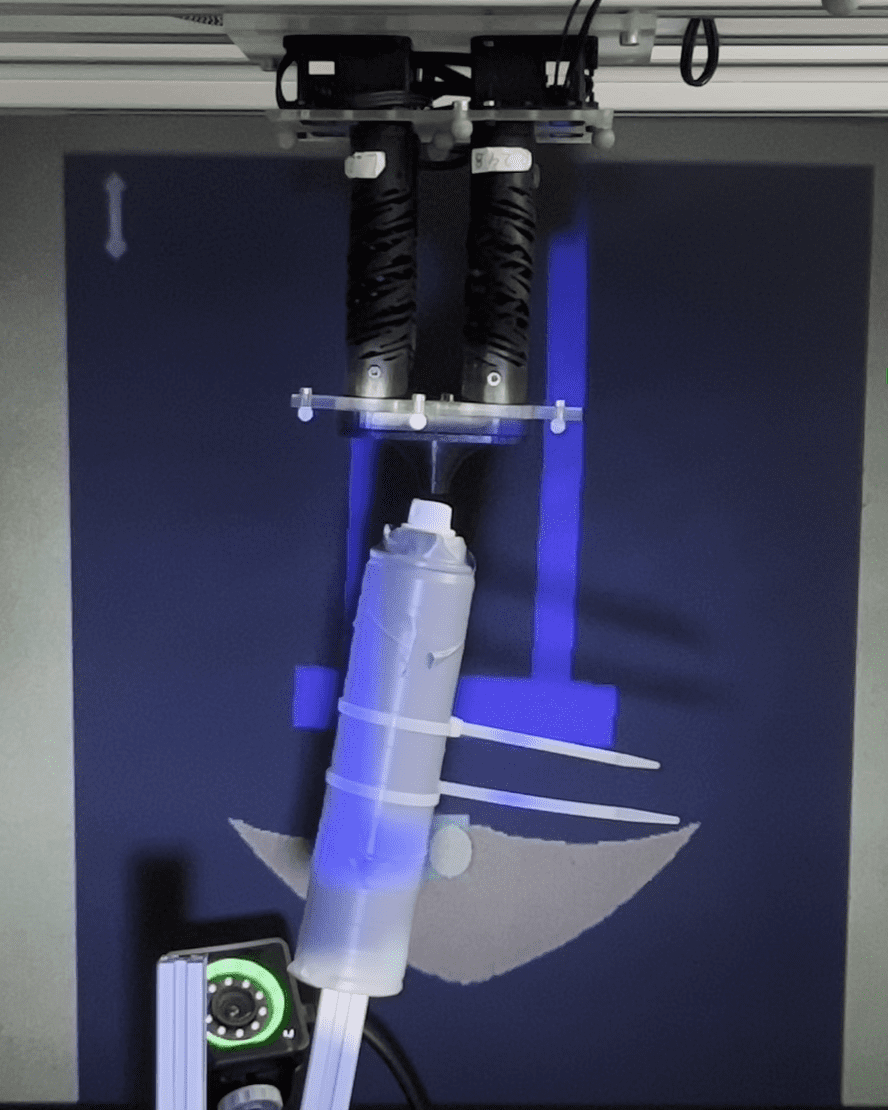
\includegraphics[width=0.192\textwidth]{braincontrol/figures/adl_task/20231031_203004_trimmed_and_cropped-0007-min.png}}
    \subfigure[$t=\SI{84}{s}$]{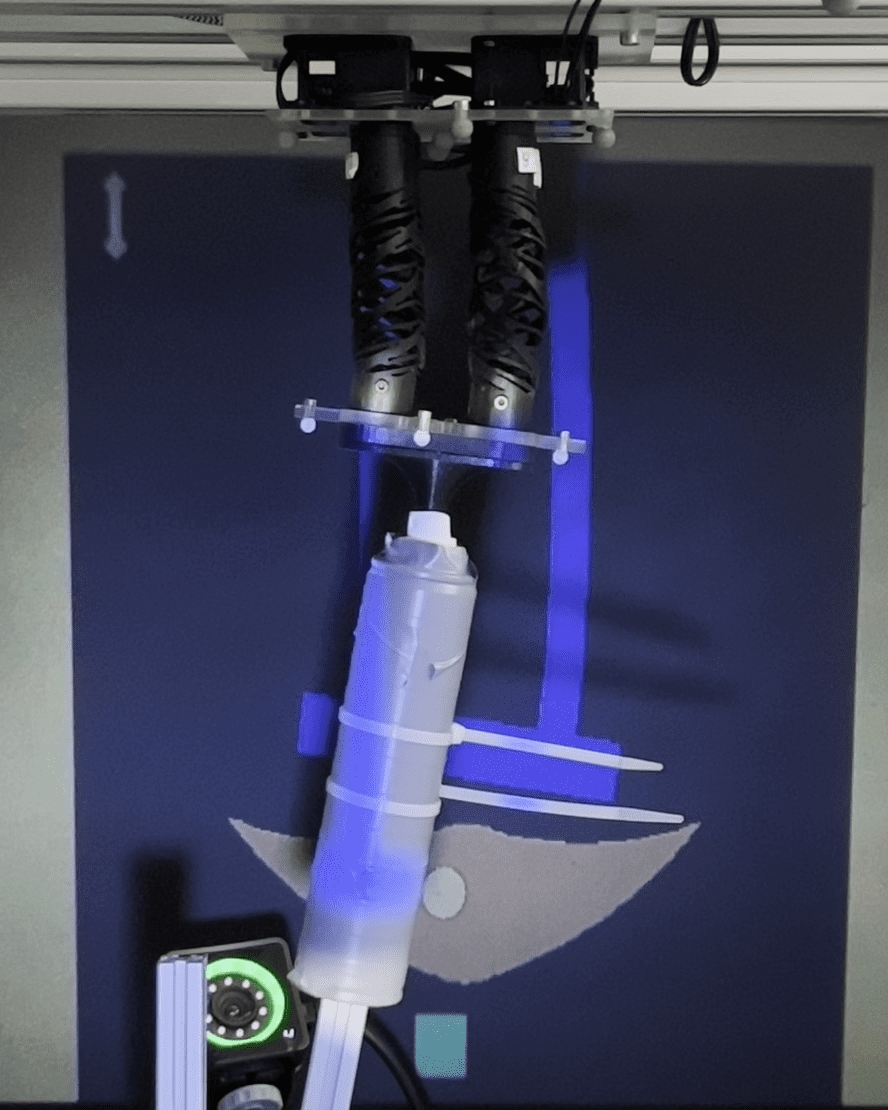
\includegraphics[width=0.192\textwidth]{braincontrol/figures/adl_task/20231031_203004_trimmed_and_cropped-0008-min.png}}
    \subfigure[$t=\SI{96}{s}$]{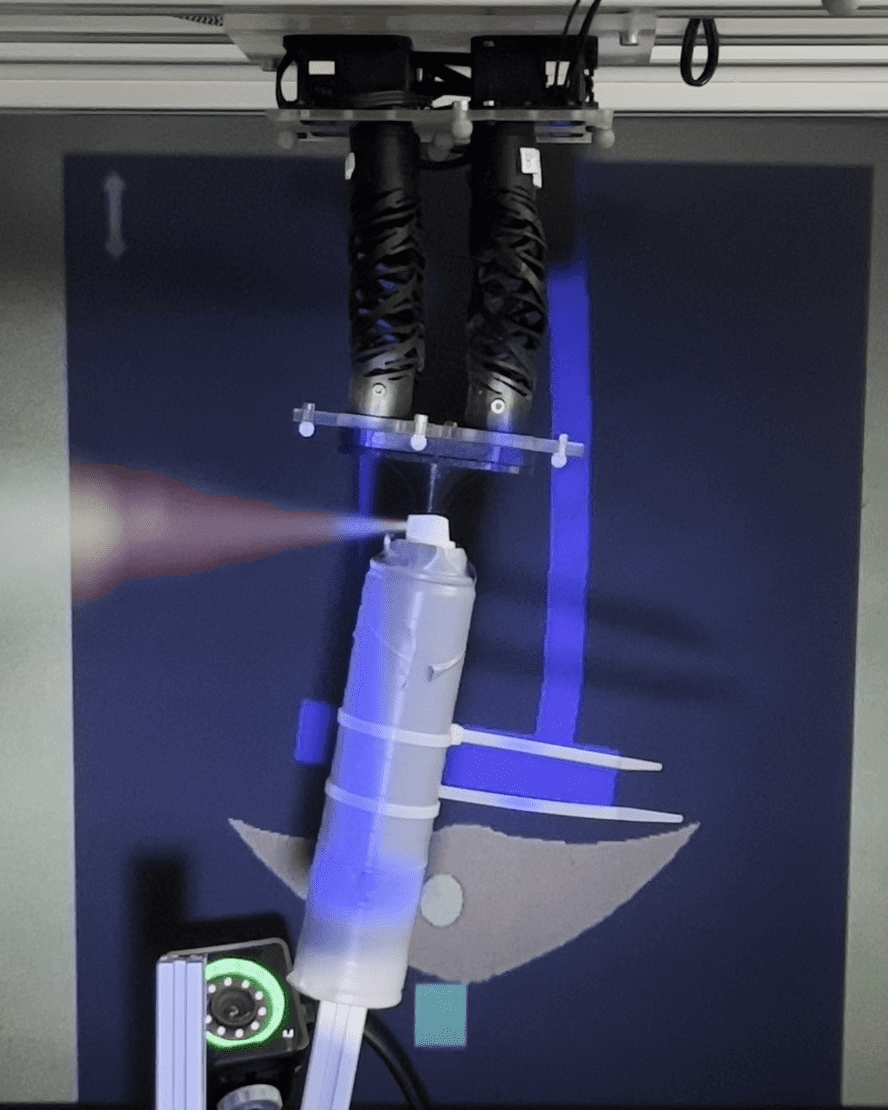
\includegraphics[width=0.192\textwidth]{braincontrol/figures/adl_task/20231031_203004_trimmed_and_cropped-0009_edited-min.png}\label{fig:braincontrol:experimental_results:adl_task_sequence_of_stills:spraying}}
    \subfigure[$t=\SI{108}{s}$]{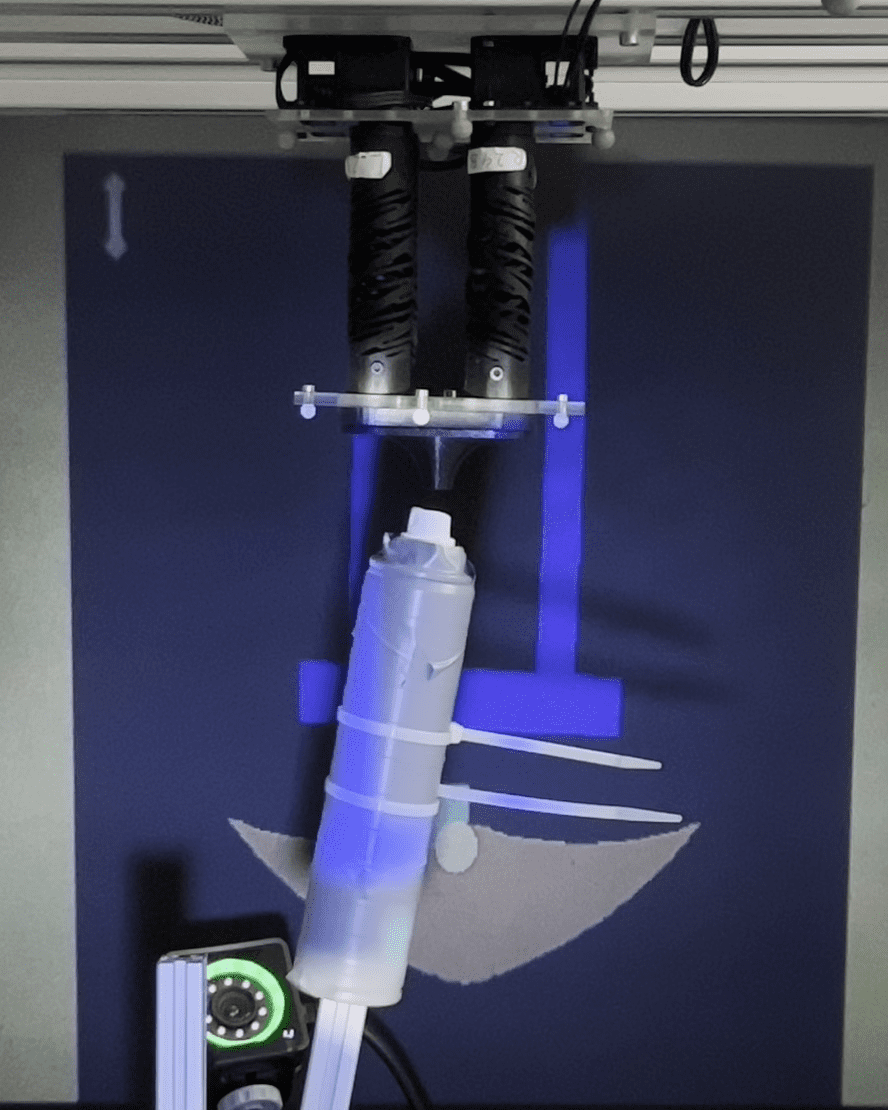
\includegraphics[width=0.192\textwidth]{braincontrol/figures/adl_task/20231031_203004_trimmed_and_cropped-0010-min.png}}
    \caption{Sequence of stills for completing a basic Activity of Daily Living (ADL) by controlling the robot with EEG-based motor imagery.
    \emph{Note: }Fig.~\ref{fig:braincontrol:experimental_results:adl_task_sequence_of_stills:spraying} is edited for improved contrast.
    }\label{fig:braincontrol:experimental_results:adl_task:sequence_of_stills}
\end{figure*}

\subsection{Interacting with the environment on a real-world task}\label{sub:braincontrol:experiments:adl}
We consider the \gls{ADL} task of releasing hairspray by actuating the button of its container with the \gls{HSA} robot's end-effector (see Fig.~\ref{fig:braincontrol:cartesian_impedance_adl}). For successful execution, the end-effector must be very stiff in the normal direction of the contact. On the other hand, we might want to benefit from the physical intelligence of the system by being relatively flexible in the tangential direction. Therefore, we first define the perpendicular stiffness $k_\perp = \SI{500}{N\per\meter}$ and the tangential stiffness as $k_\parallel = \SI{50}{N \per \meter}$. We assume that the normal direction of the contact can be described by the polar angle $\theta_\perp$ (with respect to the x-axis). We envision that in the future, the user can adjust such stiffness characteristics online via a \gls{BMI} system similar to~\citep{schiatti2017soft}. In this chapter, however, we estimate by visual inspection that $\theta_\perp=\SI{1.31}{rad}$.
The Cartesian stiffness matrix in global coordinates is then given by $K_x = R(\theta_\perp) \, \mathrm{diag}(k_\perp, k_\parallel) \, R(\theta_\perp)^\mathrm{T}$
where $R(\theta_\perp) \in SO(2)$ is the rotation matrix between global and contact frames.
% Analog to the setpoint regulation task, the user can move the attractor freely in Cartesian space when executing the described \gls{ADL} task.

\begin{figure}[hbt]
    \centering
    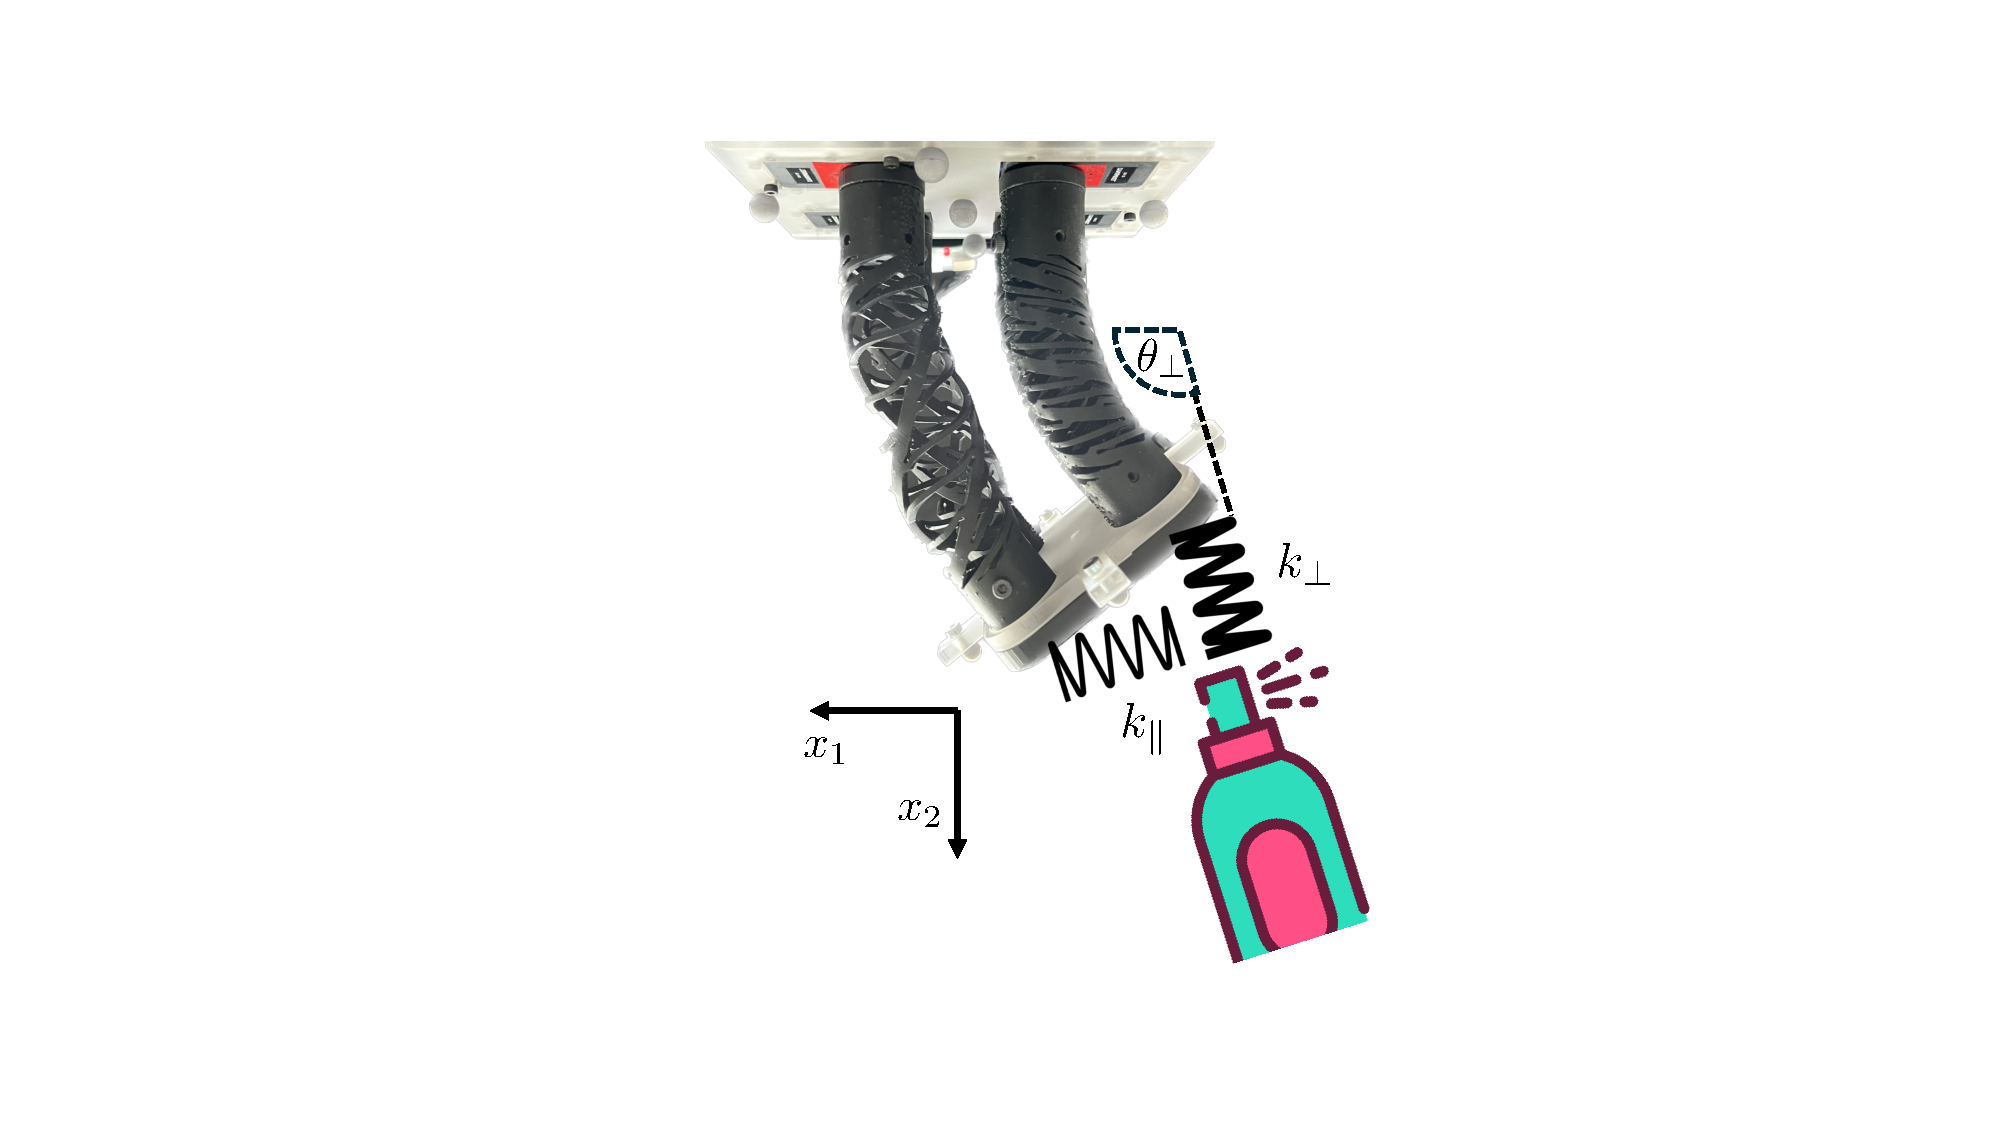
\includegraphics[width=0.35\textwidth]{braincontrol/figures/adl_task/cartesian_impedance_adl_cropped.pdf}
    \caption{Cartesian impedance shaping when interacting with the environment, for example, while performing \gls{ADL}. }
    \label{fig:braincontrol:cartesian_impedance_adl}
\end{figure}

\begin{figure}[htb]
    \centering
    \subfigure[End-effector $x$-coordinate]{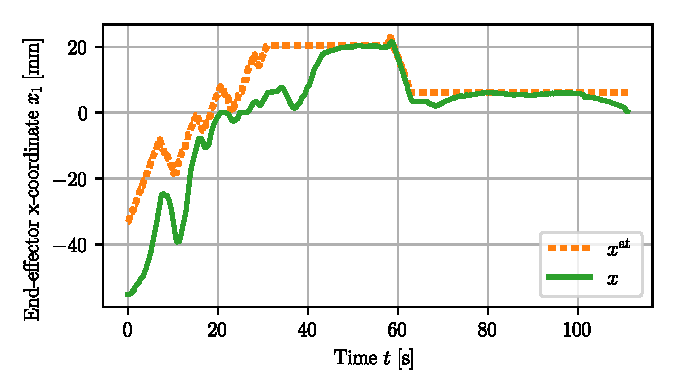
\includegraphics[width=0.47\textwidth, trim={5, 5, 5, 5}]{braincontrol/figures/adl_task/20231031_203004_pee_x.pdf}\label{fig:braincontrol:experimental_results:adl_task:brain:pee_x}}
    \subfigure[End-effector $y$-coordinate]{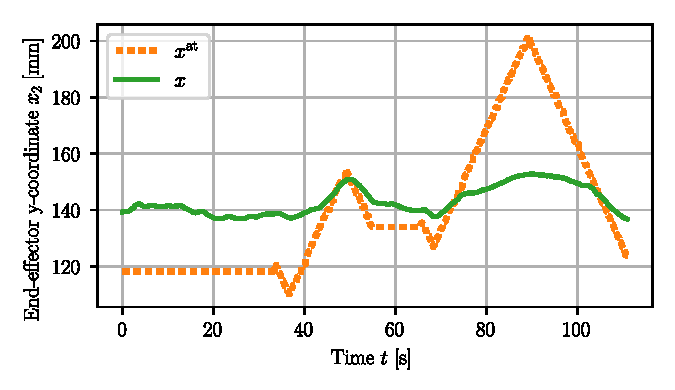
\includegraphics[width=0.47\textwidth, trim={5, 5, 5, 5}]{braincontrol/figures/adl_task/20231031_203004_pee_y.pdf}\label{fig:braincontrol:experimental_results:adl_task:brain:pee_y}}
    \\
    \subfigure[Configuration $q$]{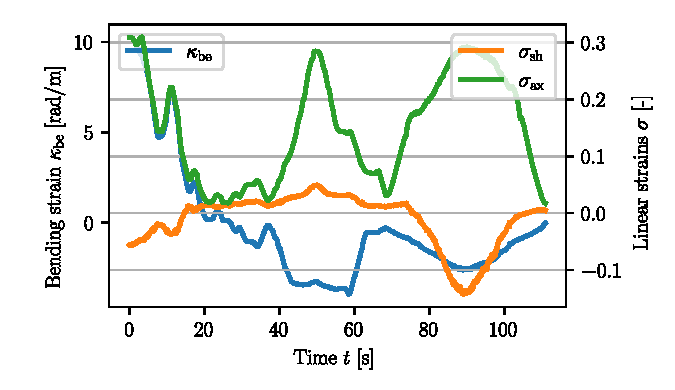
\includegraphics[width=0.47\textwidth, trim={5, 5, 5, 5}]{braincontrol/figures/adl_task/20231031_203004_q.pdf}\label{fig:braincontrol:experimental_results:adl_task:brain:q}}
    % \subfigure[Joy signal $u$]{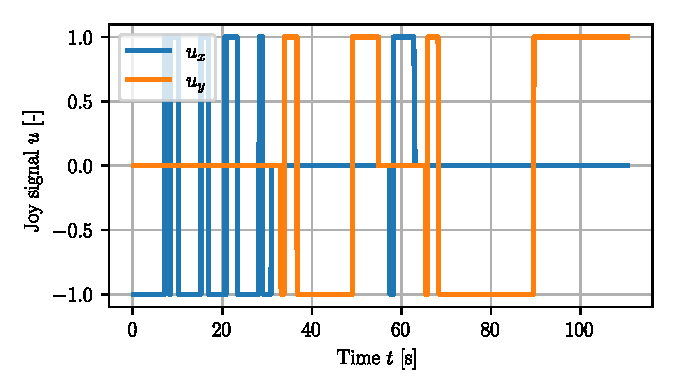
\includegraphics[width=0.49\textwidth, trim={5, 5, 5, 5}]{braincontrol/figures/adl_task/20231031_203004_joy_signal.pdf}\label{fig:braincontrol:experimental_results:adl_task:brain:u}}
    \subfigure[Control input $\phi$]{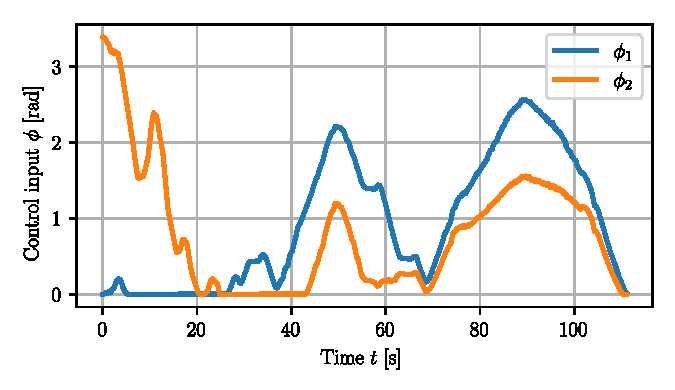
\includegraphics[width=0.47\textwidth, trim={5, 5, 5, 5}]{braincontrol/figures/adl_task/20231031_203004_phi.pdf}\label{fig:braincontrol:experimental_results:adl_task:brain:phi}}
    \caption{Experimental results for completing a basic Activity of Daily Living (ADL) by controlling the robot with EEG-based motor imagery. \textbf{Panel (a) \& (b):} The x/y-coordinate of the end-effector with the solid line and dotted lines denoting the actual and attractor position, respectively.
    \textbf{Panel (c):} The evolution of the configuration.
    % \textbf{Panel (c):} The joy commands $u$ derived from the classified brain signals used to move the attractor in Cartesian space.
    \textbf{Panel(d):} The saturated planar control inputs. }\label{fig:braincontrol:experimental_results:adl_task:brain}
\end{figure}

\subsection{Evaluation metrics}
% Look at this paper for evaluation metrics: ~\citep{rakshit2020hybrid}
In the following, we will introduce and define a few metrics that help us assess the performance of the approach.

\subsubsection{Event-Related Synchronization/De-Synchronization:}
We apply \gls{ERD} / \gls{ERS}~\citep{pfurtscheller1999event} to demonstrate the difference between \gls{EEG} signals when the participant imagines right-hand movement vs. rest, i.e., no activity. \gls{ERD}/\gls{ERS} corresponds to a shift in power during imagination with respect to a baseline. It is defined by
\begin{equation}
    \mathrm{ERD/ERS}(t, f) = \frac{P(t, f) - P_{\mathrm{base}}(f)}{P_{\mathrm{base}}(f)},
\end{equation}
where $\mathrm{ERD/ERS}(t, f)$ represents the \gls{ERD} or \gls{ERS} at a specific time $t$ and frequency $f$, $P(t, f)$ stands for the power of brain activity during imagination, and $P_\mathrm{base}(f)$ denotes the baseline power. 

\subsection{Step response metrics}
For the task of setpoint regulation, we analyze primarily two aspects: (a) is the participant able to reach the proximity of setpoint within the (generously) allotted time of \SI{60}{s}? We define the proximity of the setpoints as $\lVert x^\mathrm{d} - x(t)\rVert_2 \leq \SI{2}{mm}$. And (b) what is the response time for reaching the proximity of the setpoint for the first time?
\section{Results and Discussion}\label{sec:braincontrol:results_and_discussion}

First, we analyze the \gls{ERD}/\gls{ERS} behavior with respect to rest vs. motor imaginations in Fig.~\ref{fig:braincontrol:ERDS}. It is evident that the baseline of rest remained the same in both scenarios when the participant did not perform motor imagery, but as soon as the cue is presented at \SI{0.0}{s}, a shift in power for the right-hand motor imagery with comparison to rest state is noticeable. 

We present the results for setpoint regulation employing motor imagery in Fig.~\ref{fig:braincontrol:experimental_results:setpoint_regulation:brain}. 
We observe that the participant can reach the proximity of the setpoint within the allotted time of \SI{60}{s} six out of nine times (i.e., \SI{66.6}{\percent}).
For the successful steps, the average response time is \SI{21.5}{s}.
However, as our protocol does not contain a command to let the attractor rest, it is challenging to keep the end-effector at the setpoint and we observe oscillations, particularly with respect to the x-coordinate.
% From the results in Fig.~\ref{fig:braincontrol:experimental_results:setpoint_regulation:keyboard}, it is evident that a keyboard is a superior \gls{HMI}. It only takes the participant two setpoints to get familiar with the interface, and afterwards, the performance displayed is excellent.
% However, for instance, for people with limb impairment, or people with Spinal Cord Injury (SCI), such an interface is inaccessible and, therefore, only represents an upper bound of what we strive to achieve with \gls{BCI} systems.
In our third experiment, we ask the Cartesian impedance controller to track the setpoints directly.
The fast response time, a well-known characteristic of model-based control approaches, is evident. However, the errors in the model (for example, caused by hysteresis or unmodelled nonlinearities)~\cite{stolzle2023experimental}, together with the lack of integral action, lead to steady-state errors. % They are especially pronounced for the y-coordinate.

Finally, we consider the \gls{ADL} task of releasing hair spray using the end-effector of the \gls{HSA} robot. We present a sequence of stills in Fig.~\ref{fig:braincontrol:experimental_results:adl_task:sequence_of_stills} and plots of the entire sequence in Fig.~\ref{fig:braincontrol:experimental_results:adl_task:brain}.
Already during the first attempt, the participant can steer the end-effector toward the button, apply force, and release the fluid within \SI{86}{s}.
The impedance of the controller is clearly visible in Fig.~\ref{fig:braincontrol:experimental_results:adl_task:brain:pee_y} when the manipulator is in contact with the object at time \SI{74}{s} to \SI{104}{s}.
Also, we noticed that the end-effector does not need to be perfectly aligned with the center of the button and can still complete the task successfully due to the compliance of the closed-loop system in the tangential direction.

We noticed that the variability of setting up the \gls{EEG} device on each study participant and the \gls{EEG} sensor noise caused by external factors (e.g., floor vibrations) still pose a considerable challenge for deploying motor imagery-based tools in practice. Furthermore, subject-specific factors such as the ability to focus on imagining motor actions, mental tiredness, etc., significantly affected the performance (e.g., classification accuracy, setpoint tracking error).
\section{Conclusion}
In this chapter, we proposed to combine motor imagery-based \gls{BMI} systems with continuum soft robots. This symbiosis promises the safe and compliant operation of robots that can assist people with limb impairments in their daily lives.
While the binary motor imagery classifier achieves an accuracy of only $\approx \SI{70}{\percent}$, we demonstrated experimentally its effectiveness through assistance with an activity of daily living and safe operation.
As demonstrated in the \gls{ADL} experiment, the physical intelligence of the soft robot can compensate for errors and deviations in the output of the \gls{BMI} classifier.
% Furthermore, we introduced a Cartesian impedance controller for planar \gls{HSA} robots that can deal with the peculiar characteristics of these robots (e.g., underactuation, non-affinity in control, etc.), and allows for model-based control without interfering with the structural compliance of the system.

% For future work, we suggest running a user study that includes a diverse group of non-expert subjects, and a more diverse set of soft robots.
% Furthermore, we it would be interesting to deploy the methodology on soft robots with more \glspl{DOF}, such as, for example, the Helix soft robot~\citep{guan2023trimmed}.
% Finally, relying on \gls{SOTA} \gls{EEG} classifiers, such as CTNet~\citep{zhao2024ctnet}, might increase the classification accuracy and ultimately allow for full 3D spatial brain control of the soft robot's task space motion - including the addition of a \emph{rest} mode which would allow the end-effector to remain at a pose.
For future work, we recommend conducting a user study with a diverse group of non-expert participants and incorporating a broader range of soft robots. Connected, it would be interesting to apply this methodology to soft robots with more \glspl{DOF}, such as the Helix soft robot~\citep{guan2023trimmed}. Finally, utilizing \gls{SOTA} \gls{EEG} classifiers like CTNet~\citep{zhao2024ctnet} could improve classification accuracy and ultimately enable full 3D spatial brain control of the soft robot’s task space motion—including the addition of a \emph{rest} mode to keep the end-effector at a fixed pose.
